\documentclass[9pt]{beamer}
\usetheme{Madrid}
\usepackage{mathtools}
\usepackage{bm}
\usepackage{esvect}
\usepackage{amsmath}
\usepackage{physics}
\usepackage{empheq}
\usepackage[many]{tcolorbox}

%$\vv{\bm{L}}

\title{Majorana's Beach}
  
\author{J.J. G\'omez Cadenas}
 
\institute{Donostia International Physics Center (DIPC)} % (optional)
 
\date[November 22, 2021] % (optional)
{Caltech in Meta Space, 22 November 2021}
 
\logo{
\includegraphics[height=0.5cm]{dipc.png}

\includegraphics[height=0.5cm]{IB.png}

\includegraphics[height=1.1cm]{erc.png}}


\tcbset{highlight math style={enhanced,
  colframe=red!60!black,colback=yellow!50!white,arc=4pt,boxrule=1pt,
  }}

\newtcbox{\mybox}[1][]{nobeforeafter,math upper,tcbox raise base,
  enhanced,frame hidden,boxrule=0pt,interior style={top color=green!10!white,
  bottom color=green!10!white,middle color=green!50!yellow},
  fuzzy halo=1pt with green,drop large lifted shadow,#1}

  
\begin{document}
\titlepage

\begin{frame}
\frametitle{Outline}
\tableofcontents
\end{frame}

\section{Neutrinos}

%
\begin{frame}
\frametitle{The beta decay situation}
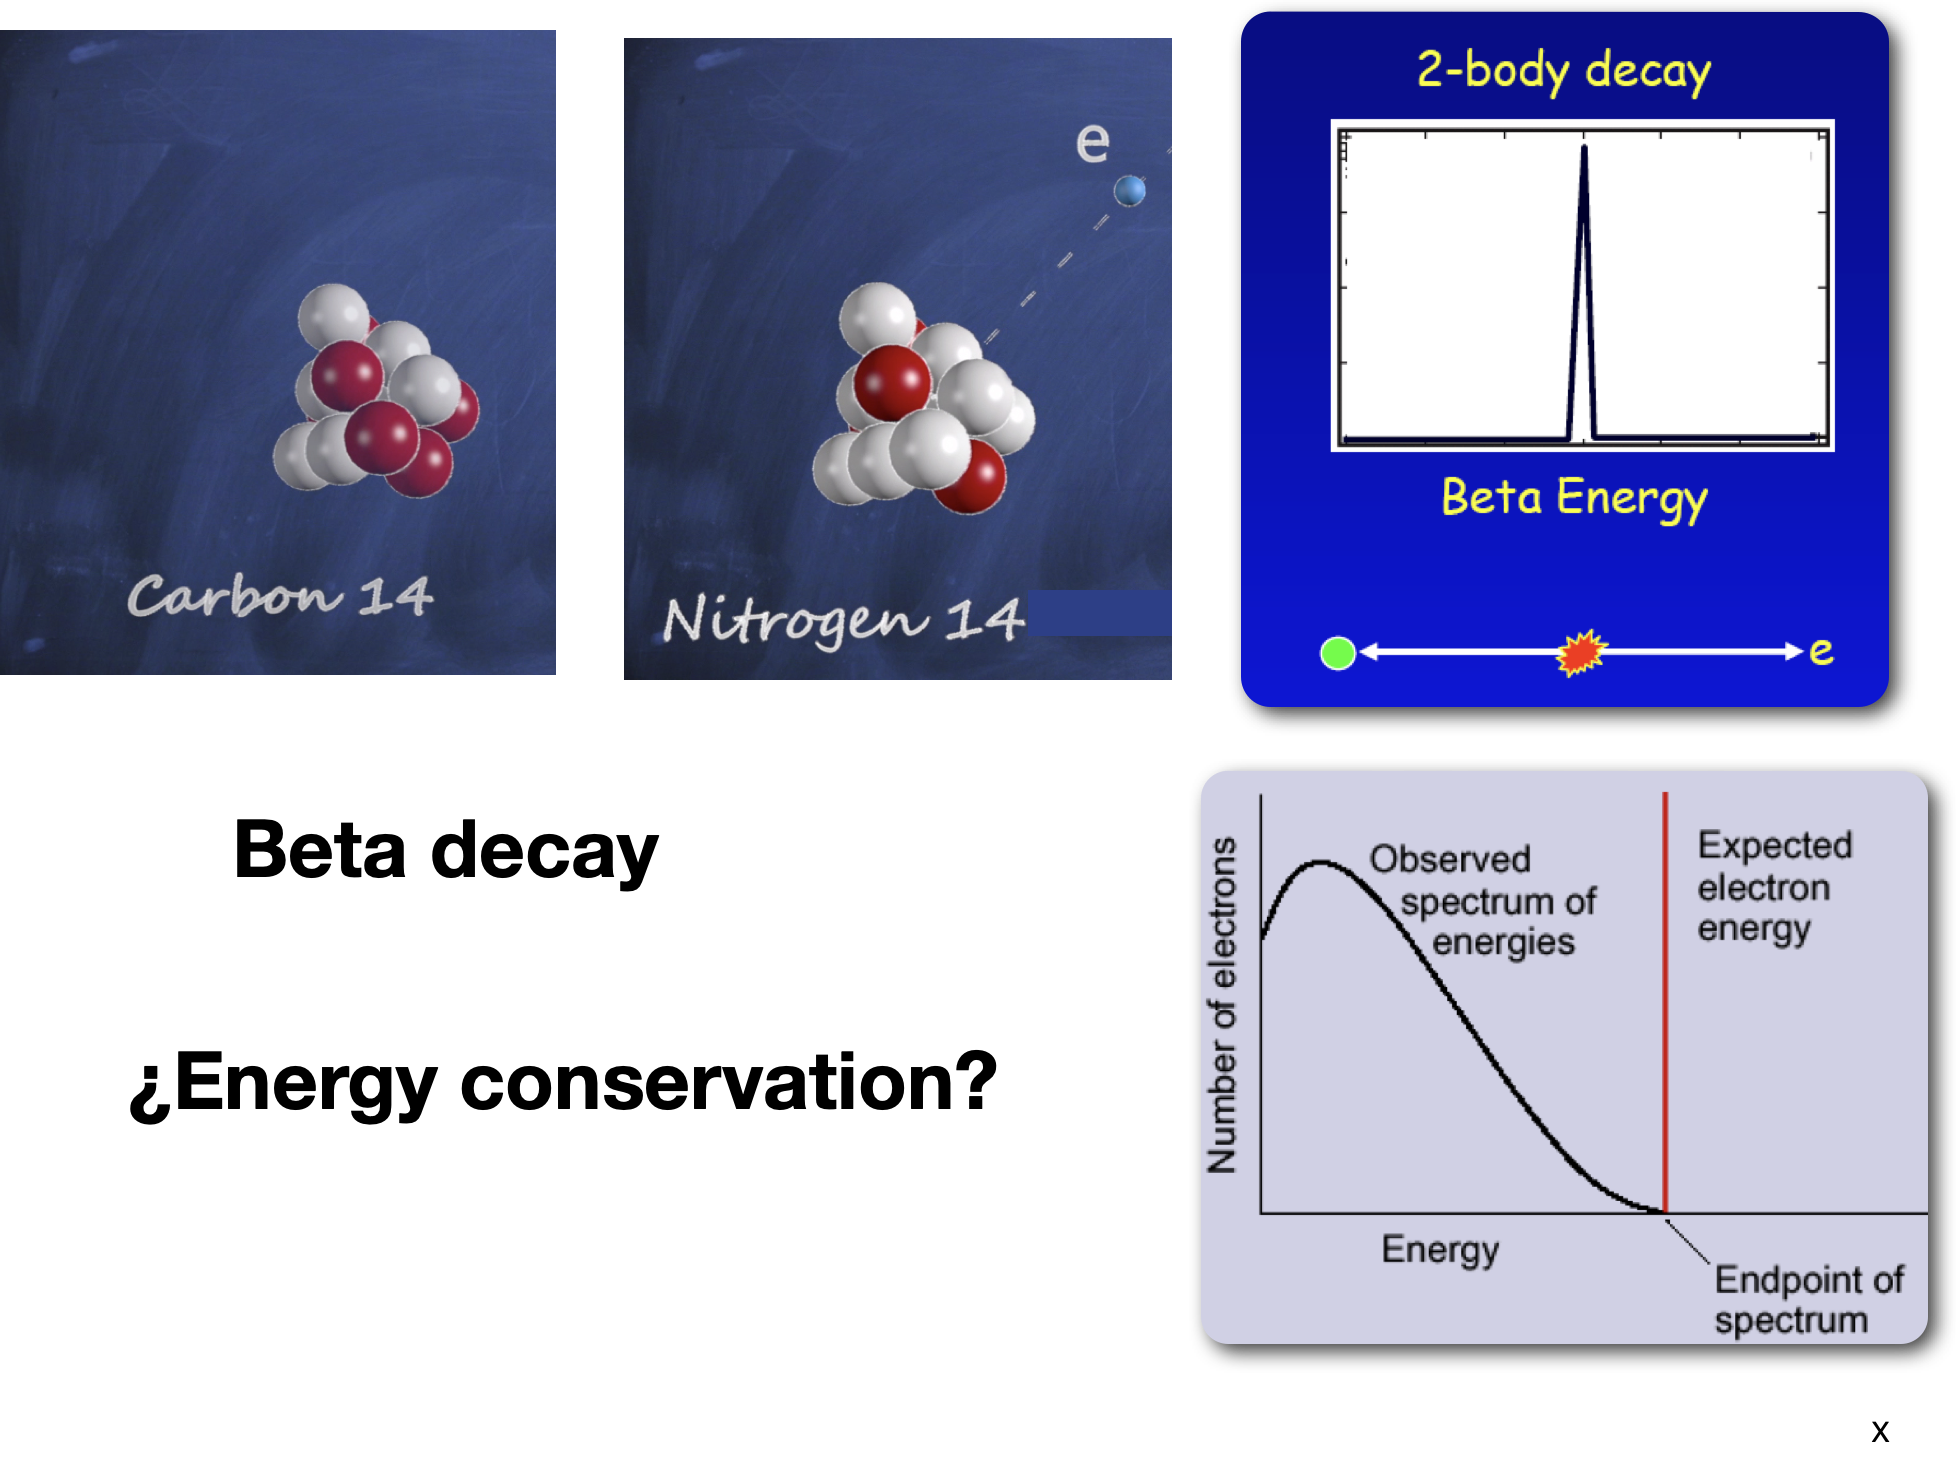
\includegraphics[scale=0.3]{img/betaDecay.png}
\end{frame}

\begin{frame}
\frametitle{Liebe Radioaktive Damen und Herren}
\begin{columns}
 
\column{0.5\textwidth}
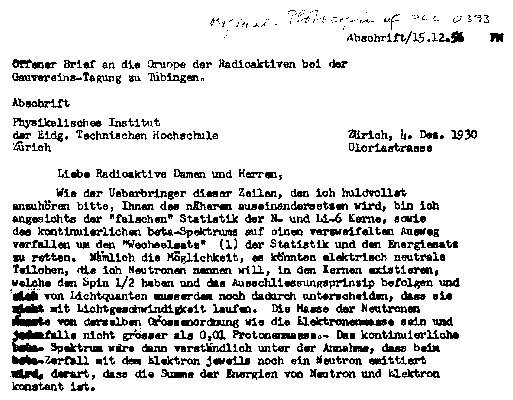
\includegraphics[scale=0.4]{img/liebe.png}
 
\column{0.2\textwidth}
\begin{block}{}
Dear Radioactive Ladies and Getlemen.

...because the continuous beta spectrum...I have hit upon a desperate remedy to save the law of conservation of energy.

\end{block}
\end{columns}
\end{frame}


%\begin{frame}
\frametitle{I do not believe in neutrinos}
\begin{columns}
\column{0.35\textwidth}
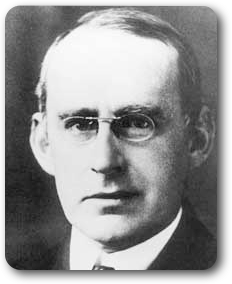
\includegraphics[scale=0.3]{img/eddington.png}
 
 \column{0.6\textwidth}
%\begin{block}{}
Sir Arthur Eddington: ``Just now nuclear physicists are writing a great deal about hypothetical particles called neutrinos supposed to account for certain peculiar facts observed in $\beta$-ray disintegration. We can perhaps best describe the neutrinos as little bits of spin-energy that have got detached. I am not much impressed by the neutrino theory. \alert{In an ordinary way I might say that I do not believe in neutrinos}... But I have to reflect that a physicist may be an artist, and you never know where you are with artists. My old-fashioned kind of disbelief in neutrinos is scarcely enough. \alert{Dare I say that experimental physicists will not have sufficient ingenuity to make neutrinos?"}

%\end{block}
\end{columns}
\end{frame}

\begin{frame}
\frametitle{The discovery of neutrinos}

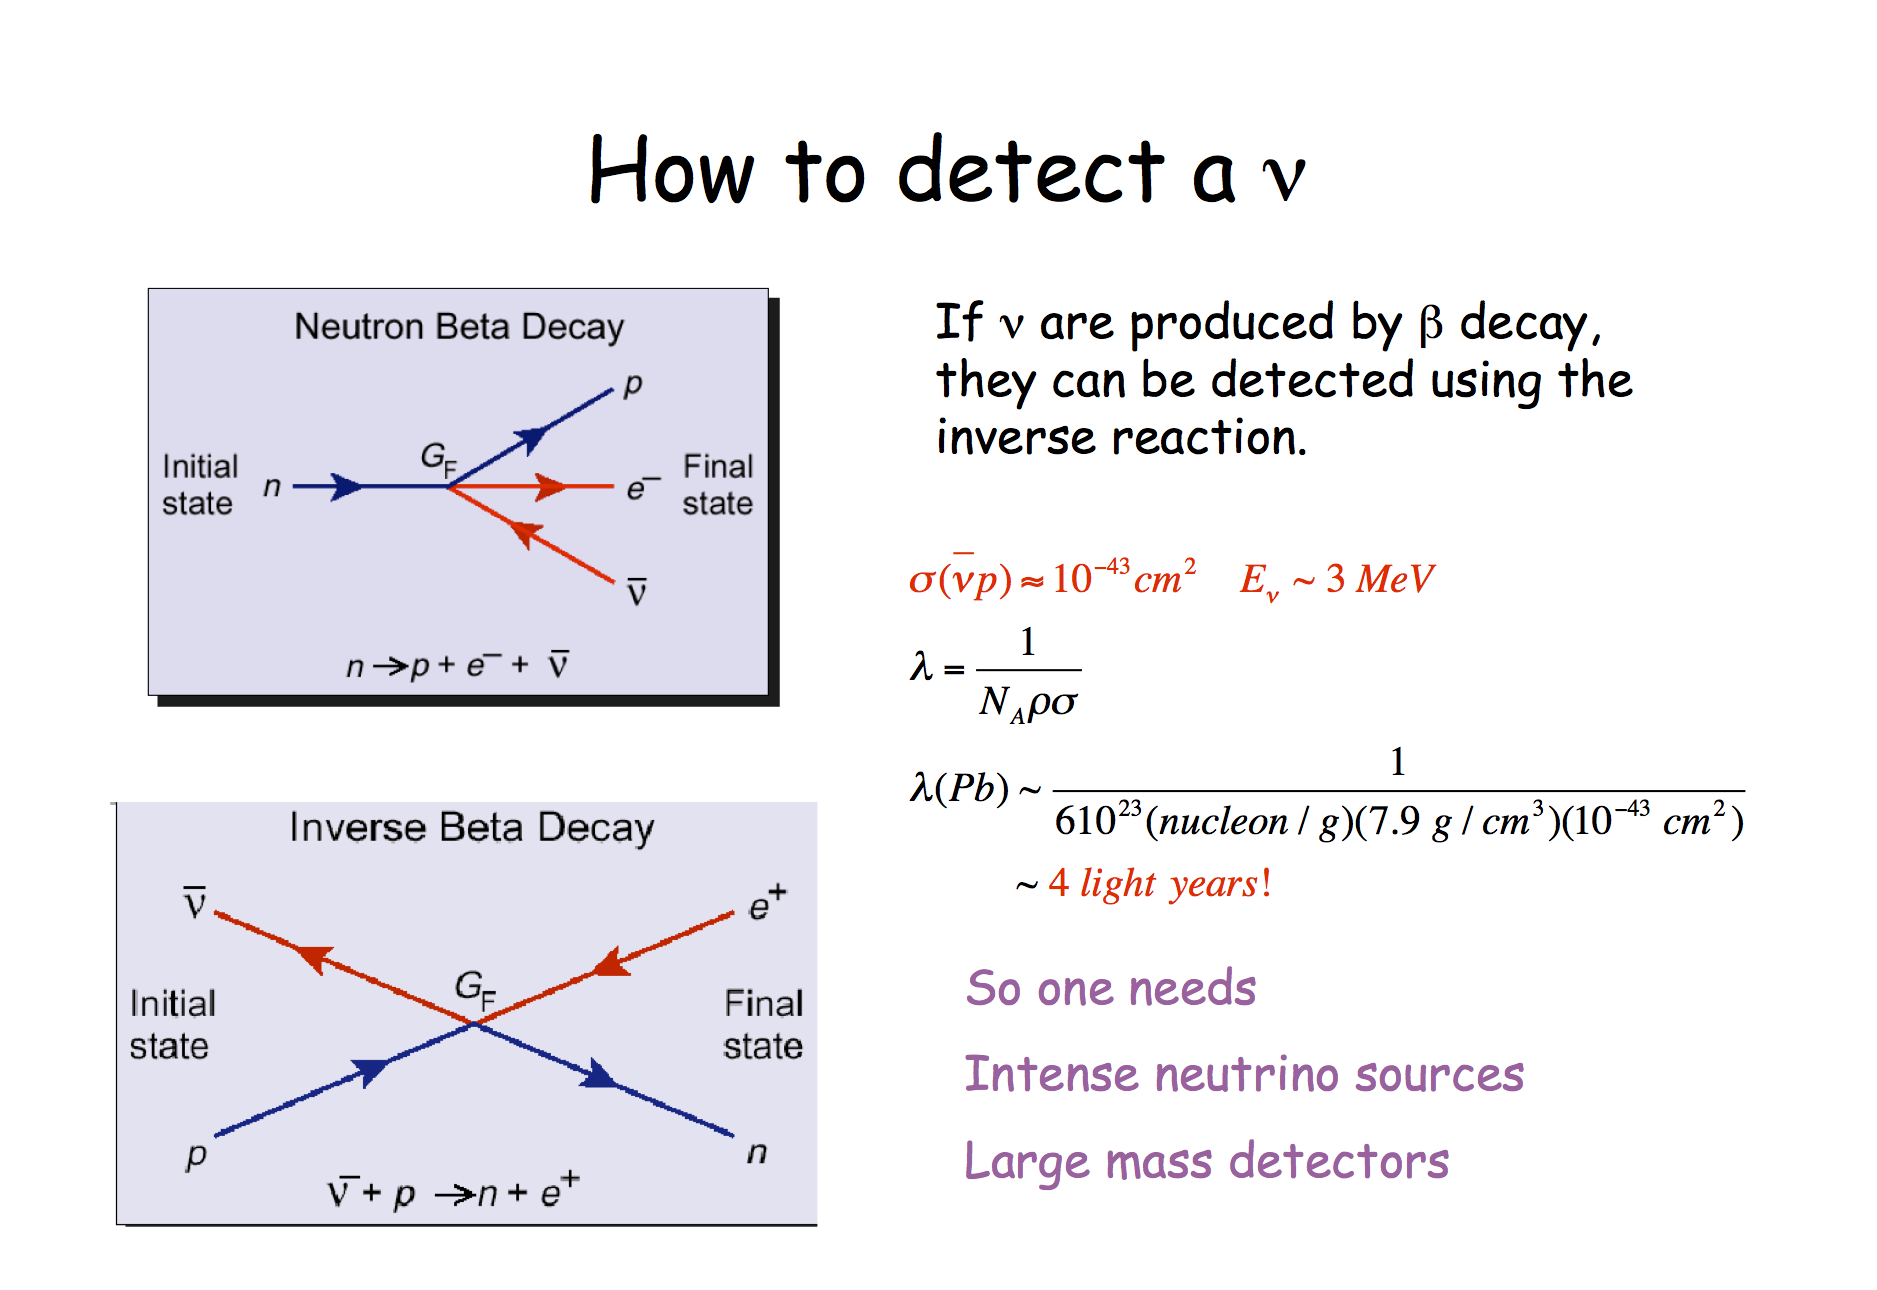
\includegraphics[scale=0.3]{img/DetectNeutrinos.png}

\end{frame}

\begin{frame}

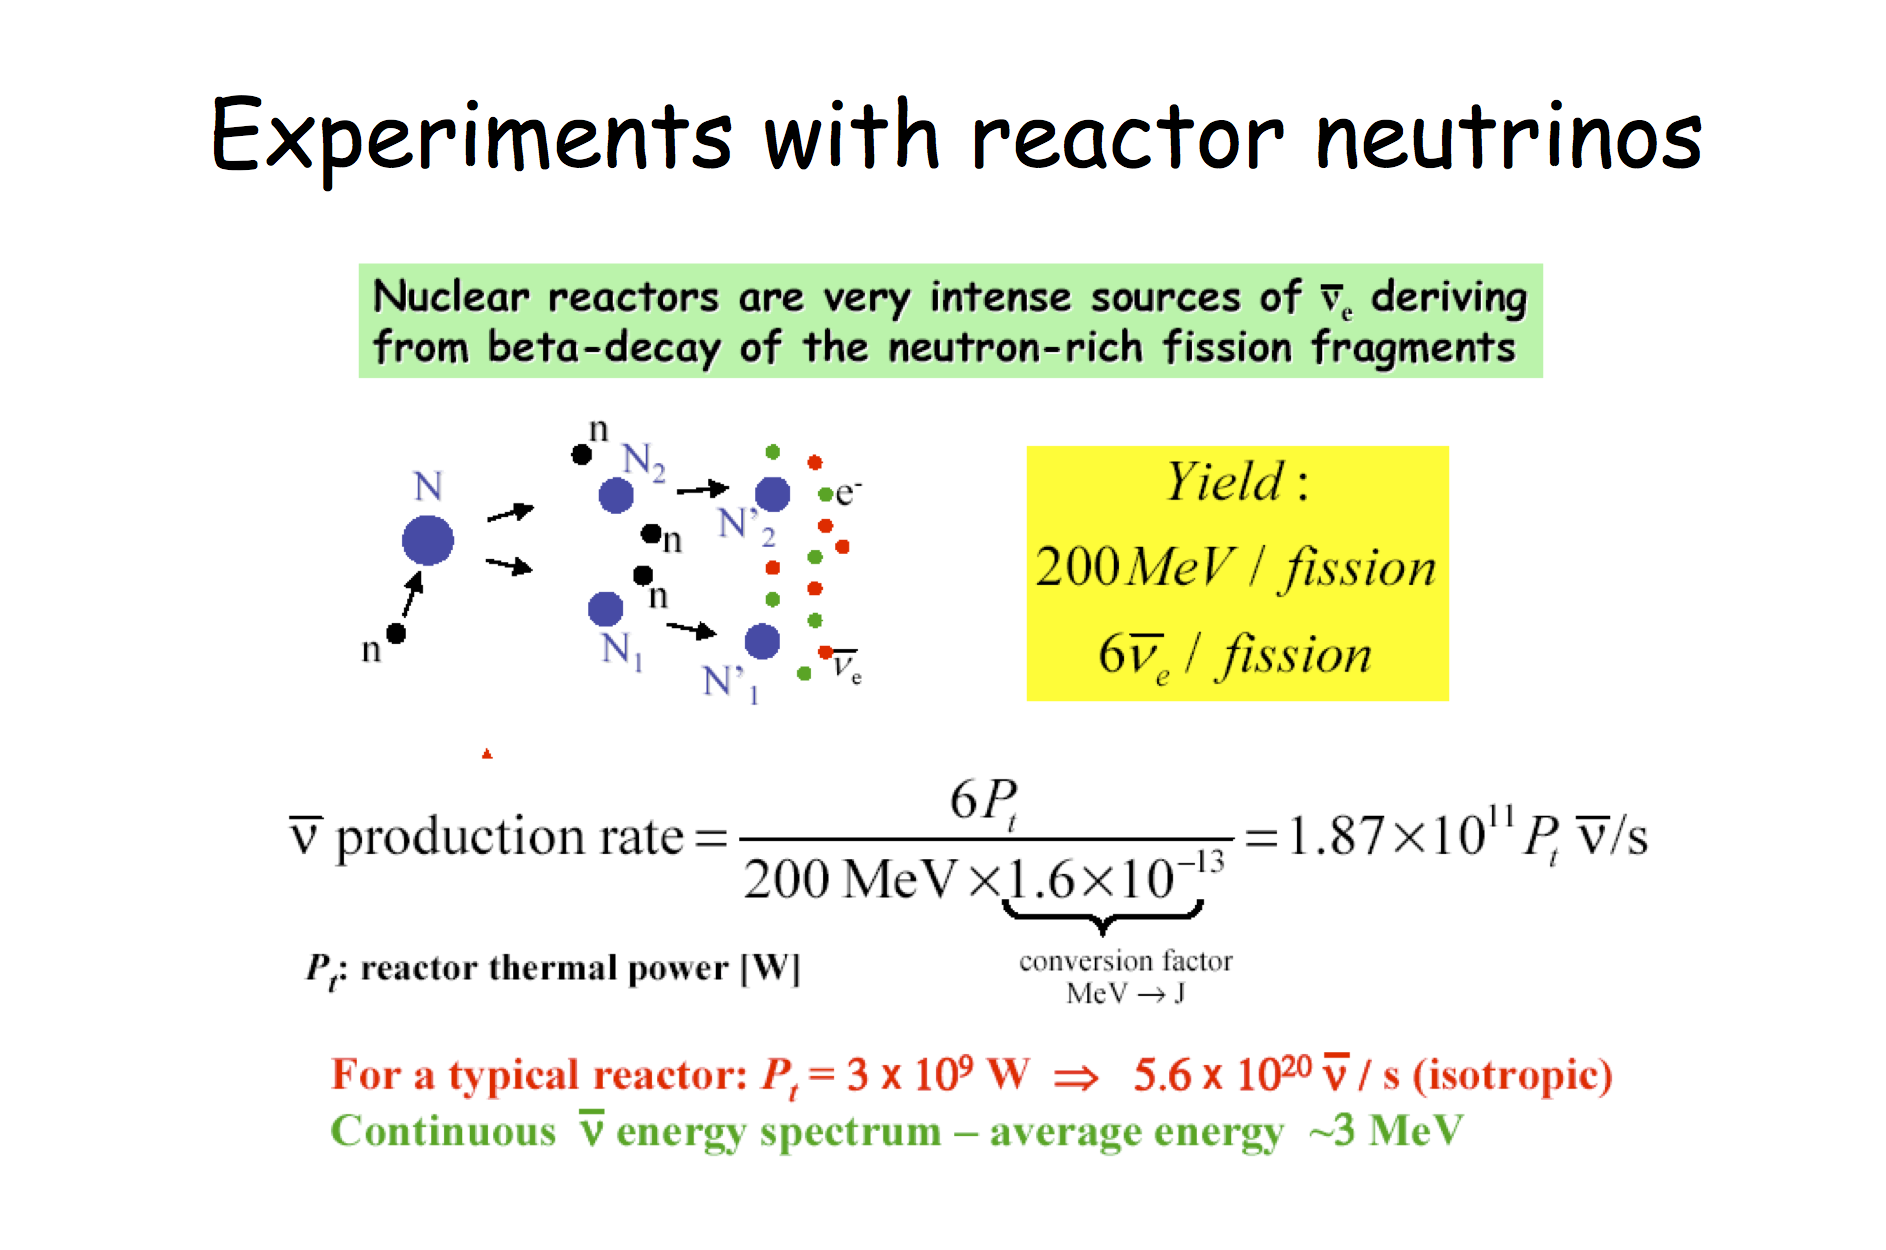
\includegraphics[scale=0.35]{img/ReactorNeutrinos.png}

\end{frame}

\begin{frame}
\frametitle{Reines, Cowen and delayed neutrons}
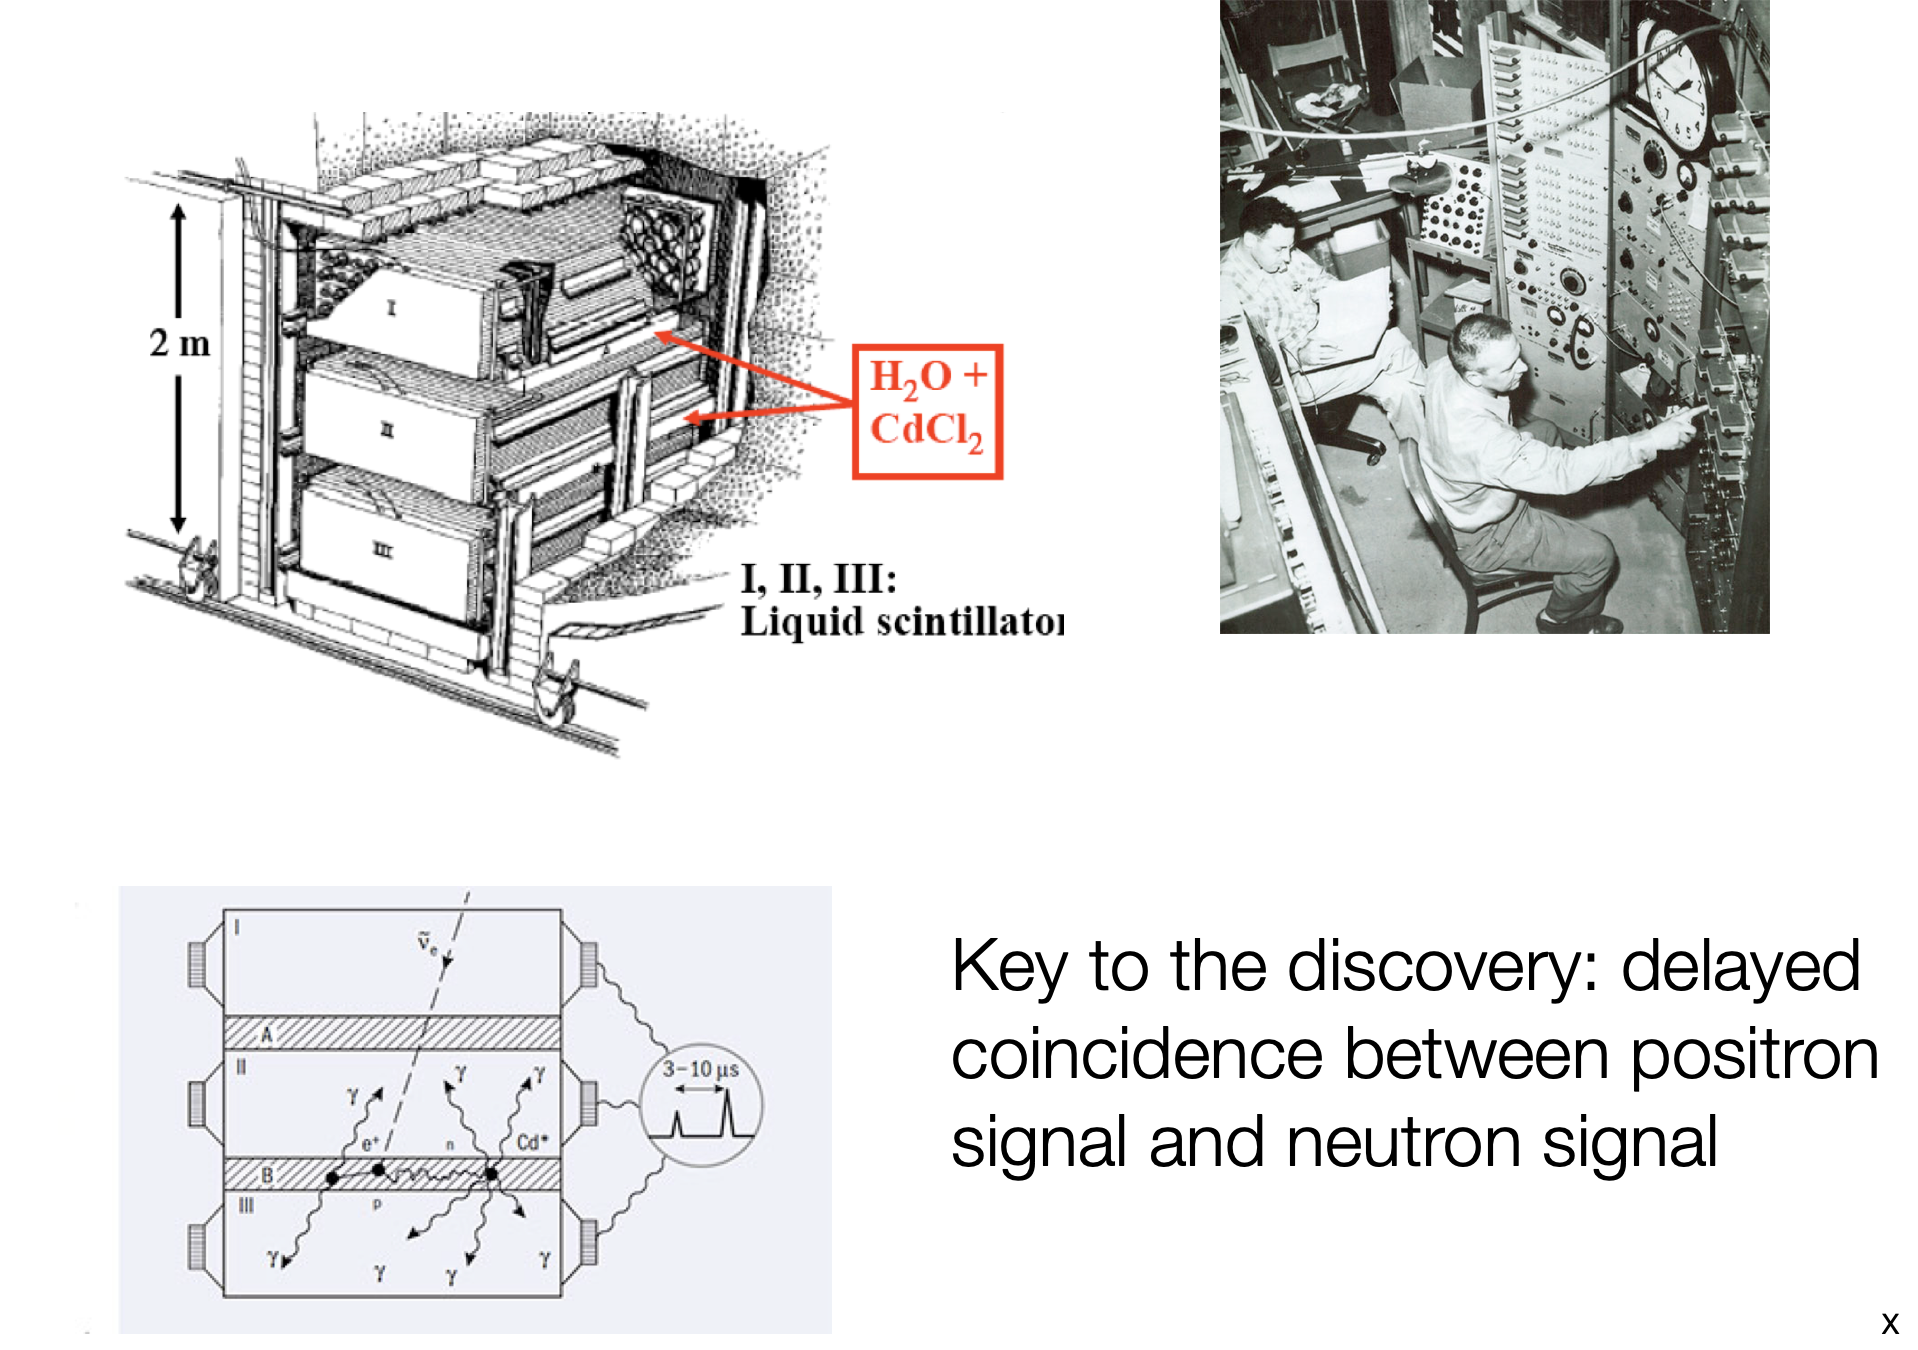
\includegraphics[scale=0.35]{img/ReinesCowen.png}

\end{frame}

%\begin{frame}
%
%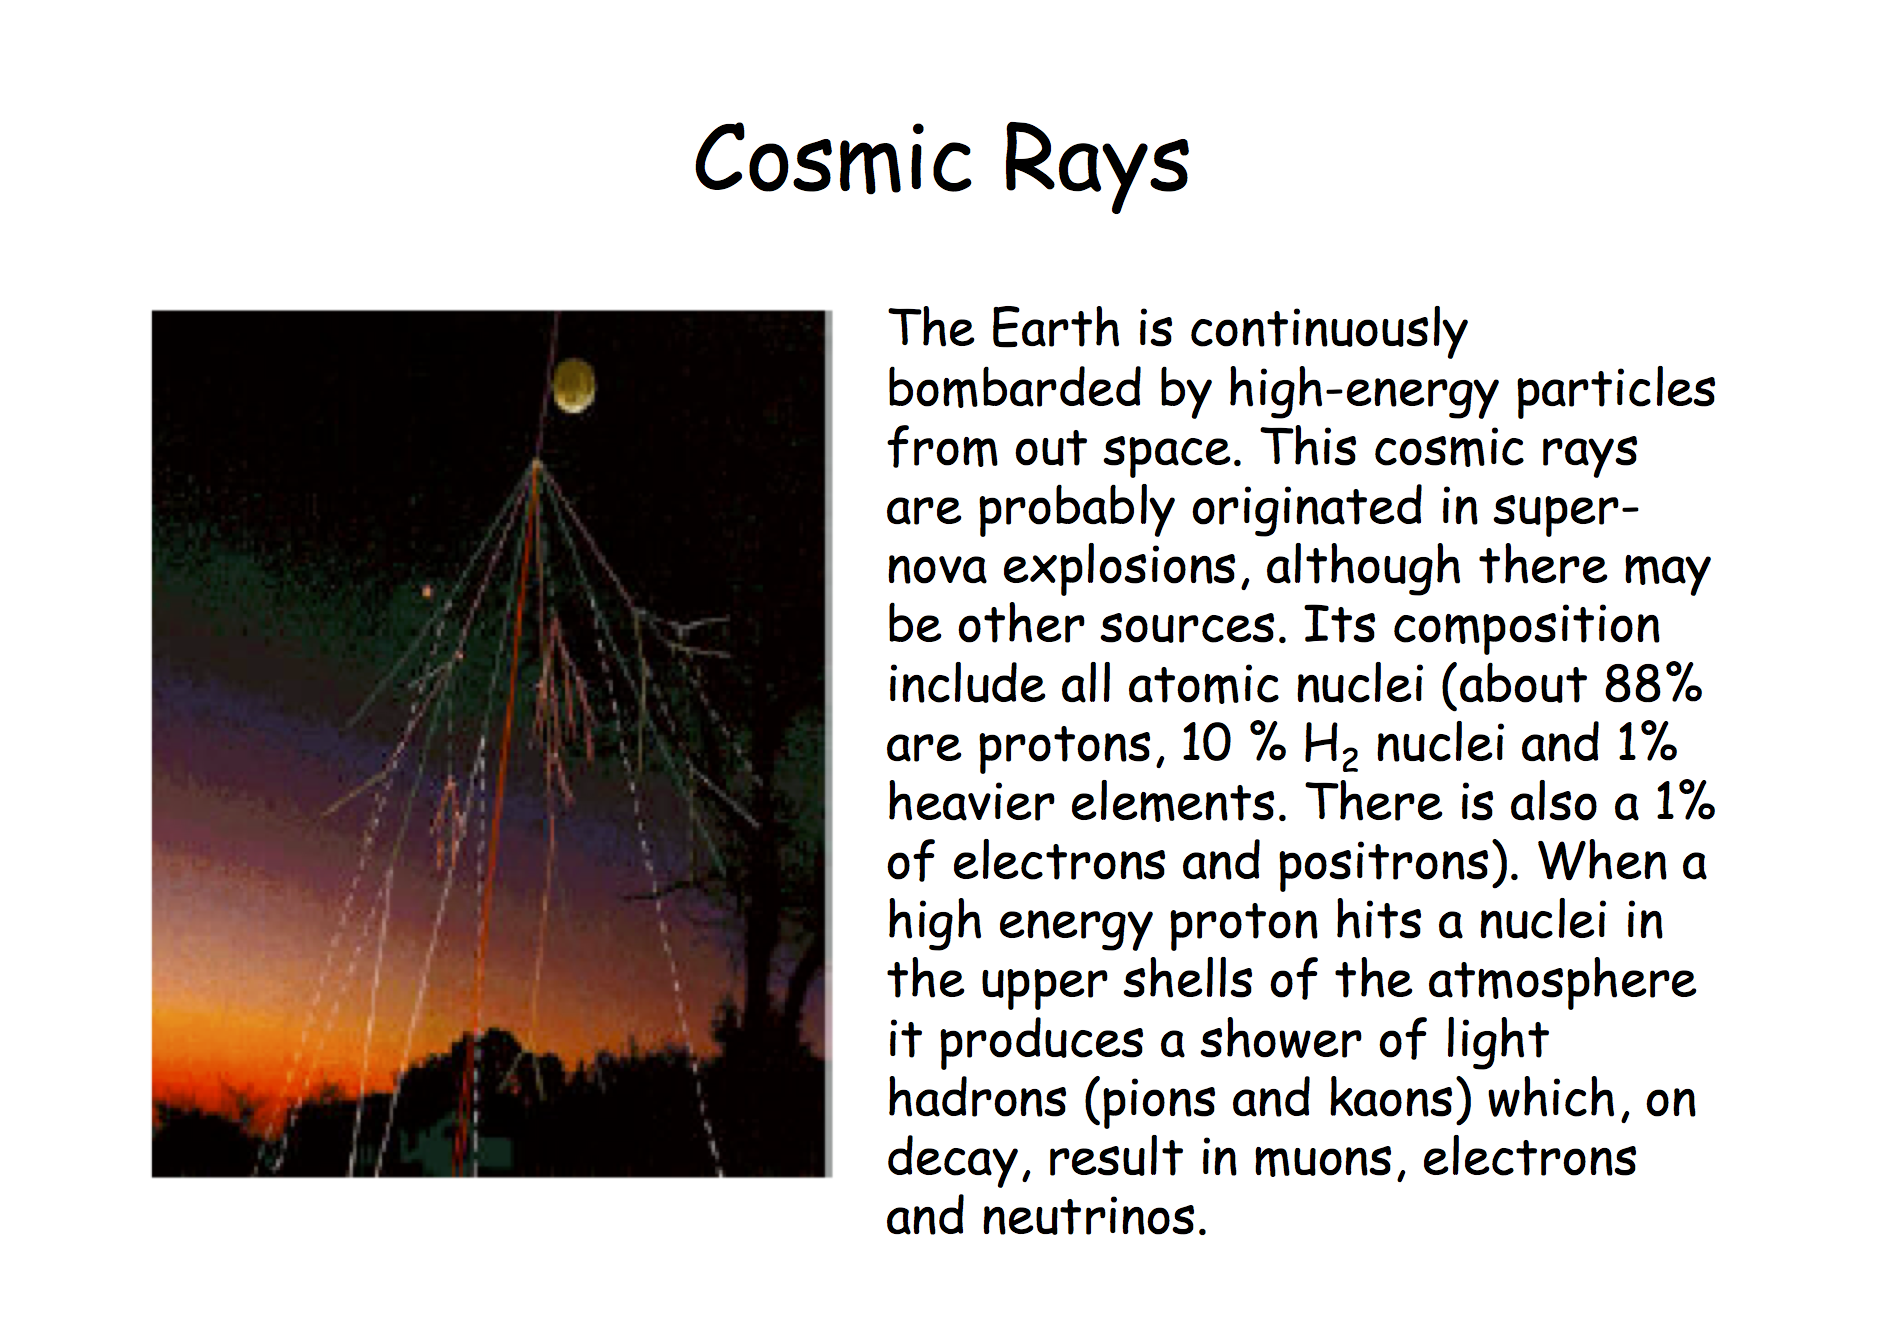
\includegraphics[scale=0.35]{CosmicRays.png}
%
%\end{frame}
%\begin{frame}
%
%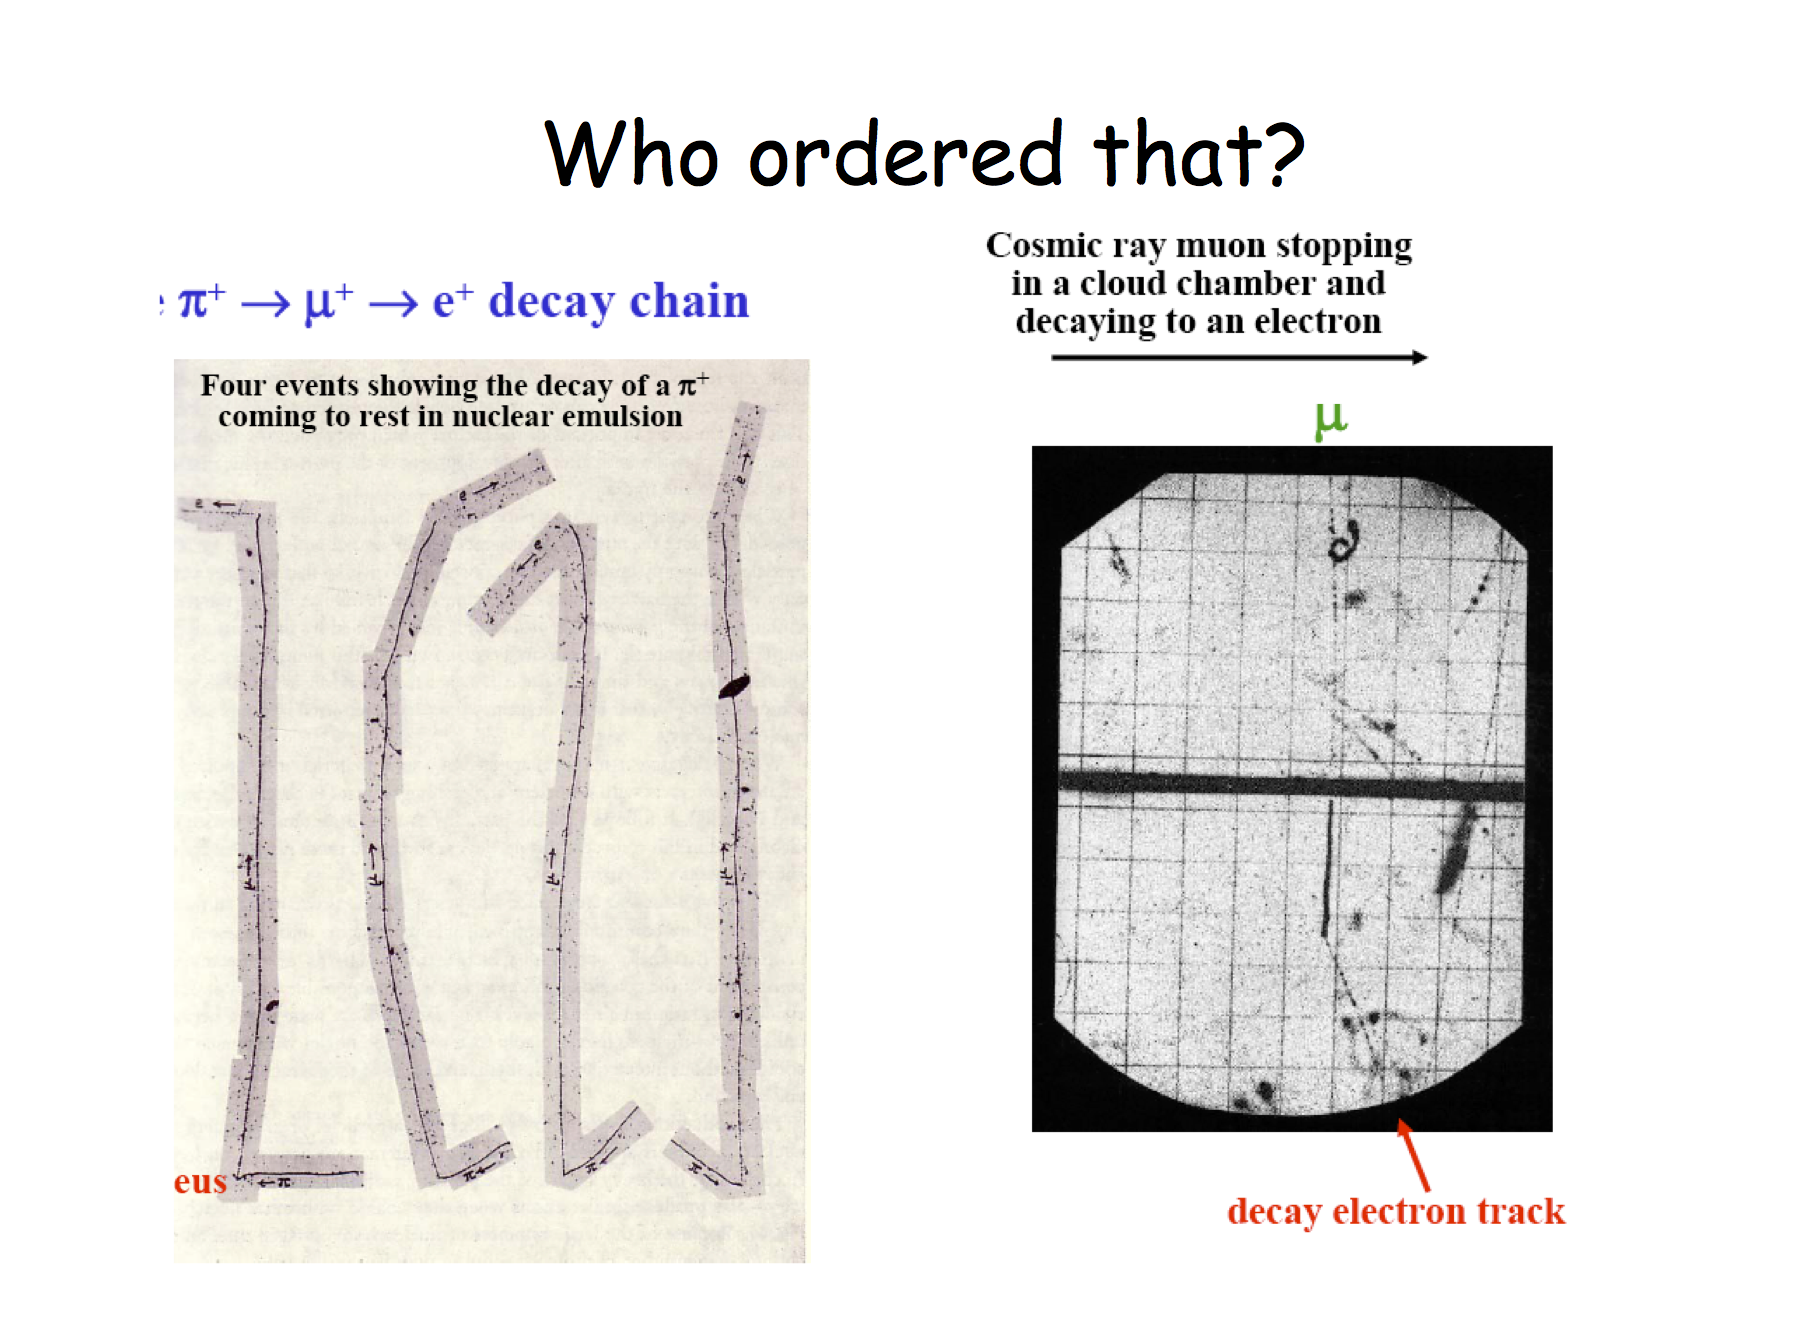
\includegraphics[scale=0.35]{WhoOrderedThat.png}
%
%\end{frame}
%\begin{frame}
%
%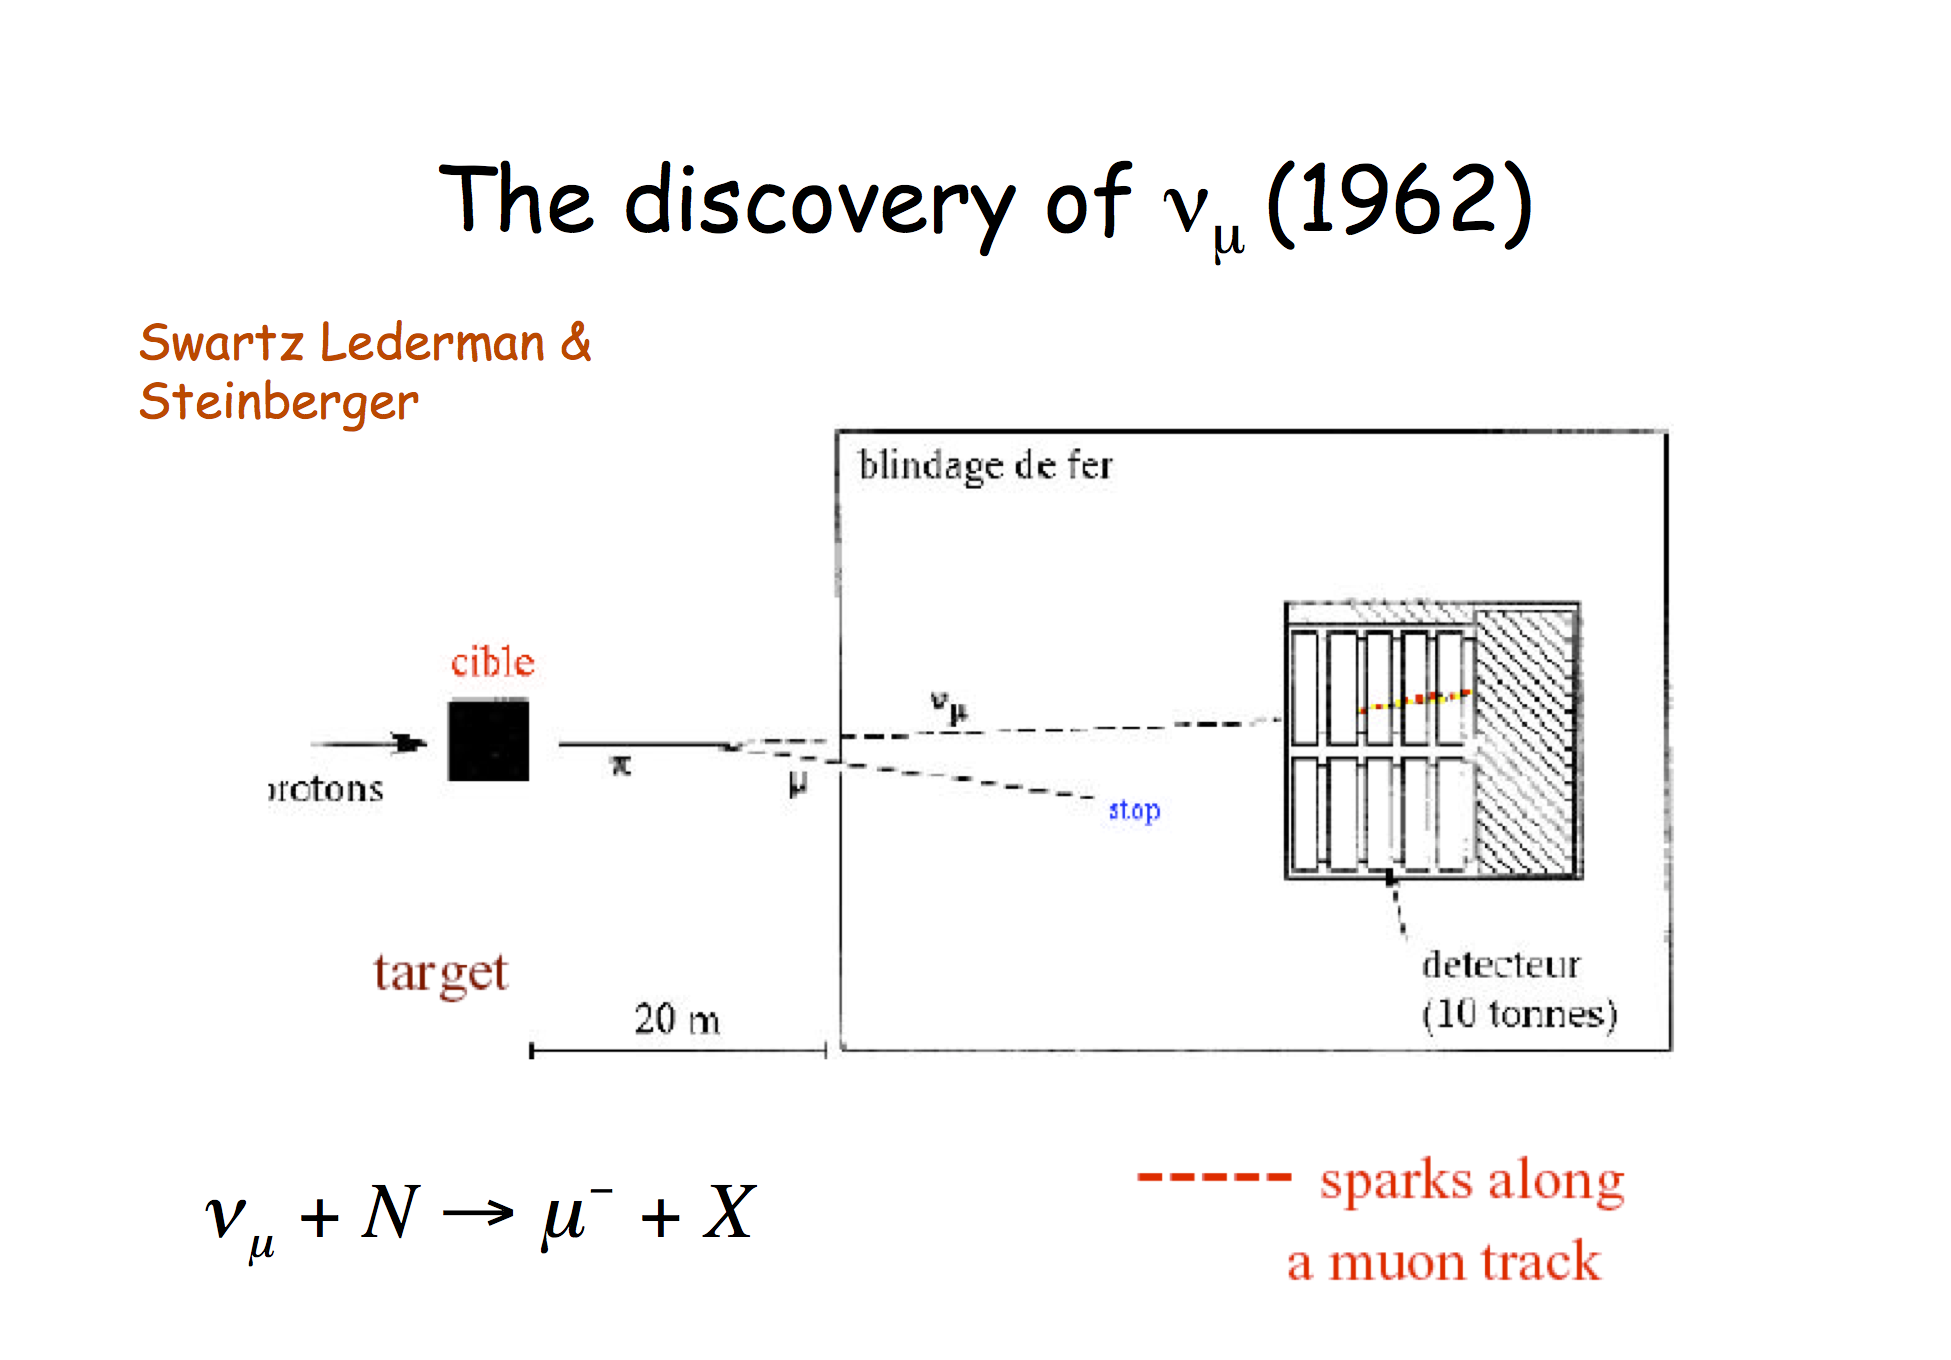
\includegraphics[scale=0.35]{DiscoveryNumu.png}
%
%\end{frame}
%\begin{frame}
%
%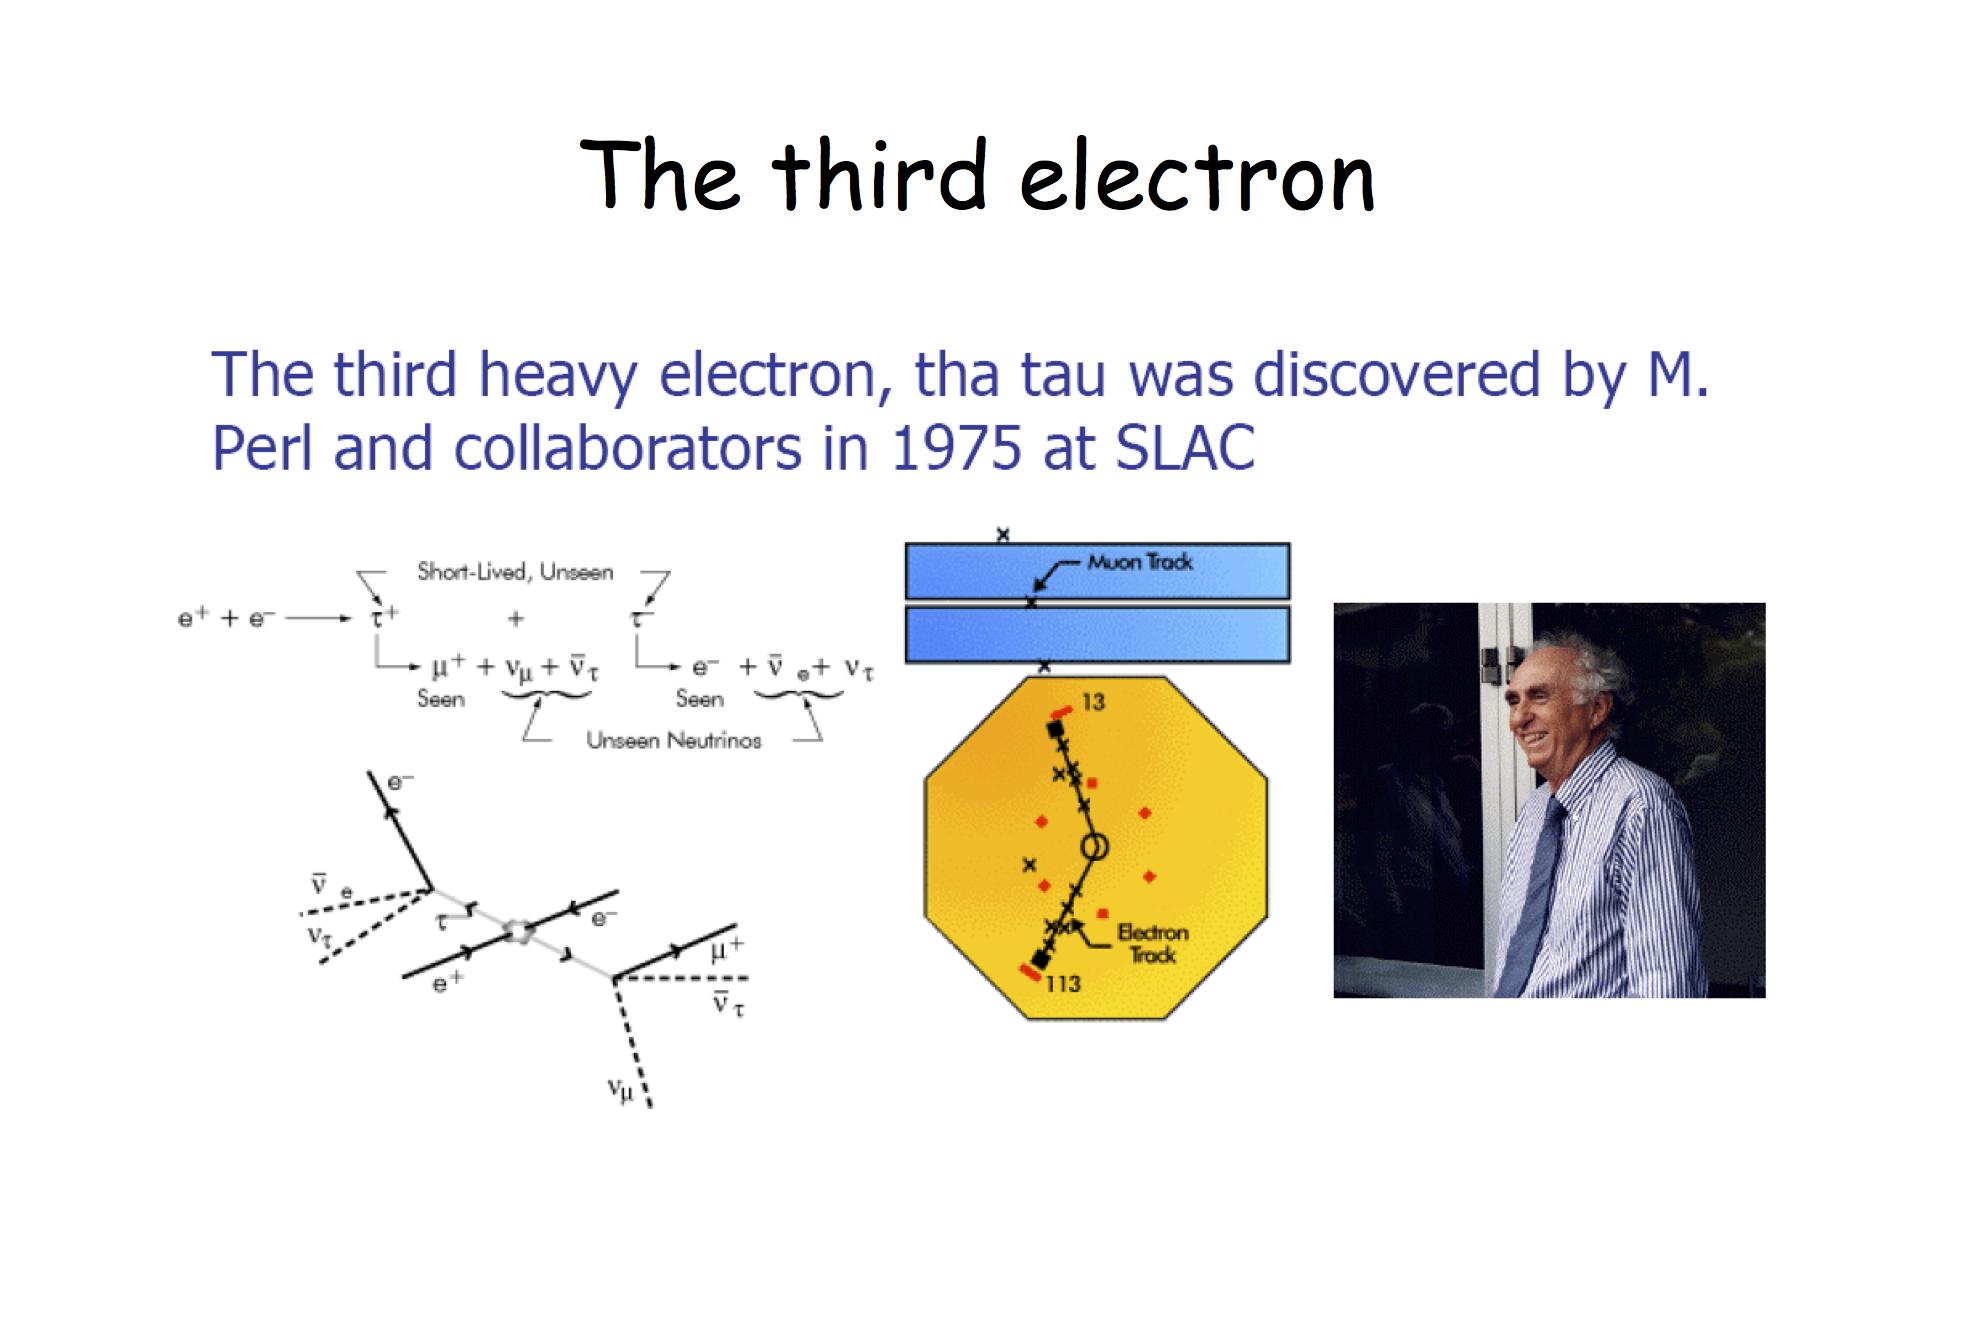
\includegraphics[scale=0.35]{tau.png}
%
%\end{frame}
%\begin{frame}
%
%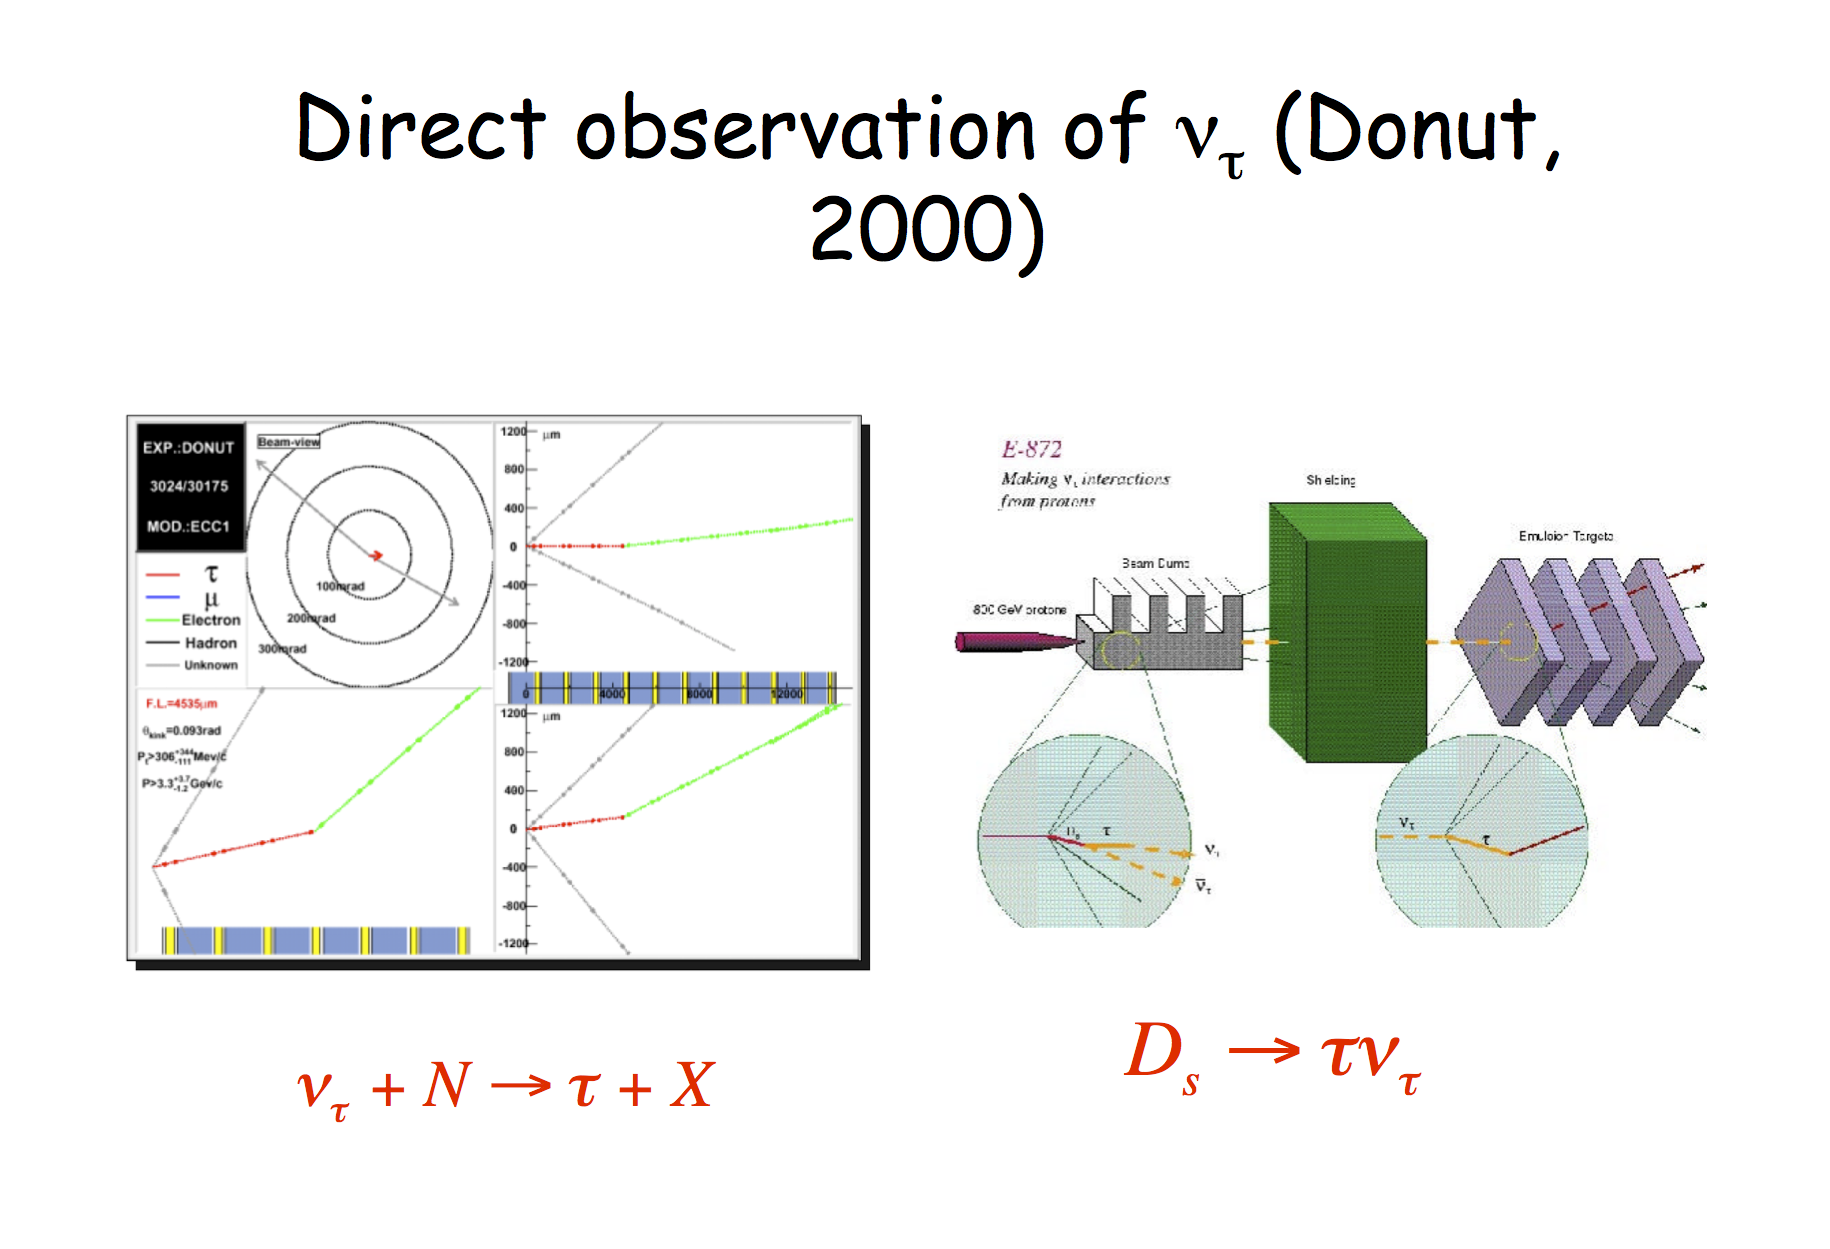
\includegraphics[scale=0.35]{DirectNuTau.png}
%
%\end{frame}
\begin{frame}
\frametitle{Neutrinos everywhere}
\begin{columns}
\column{0.35\textwidth}
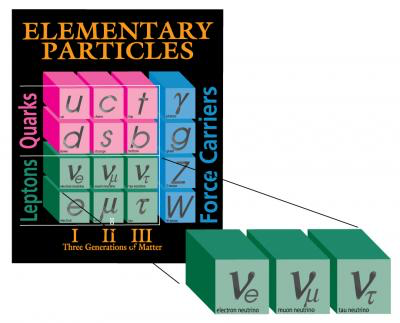
\includegraphics[scale=0.25]{img/Generations2.png}

Two heavy electrons (the $\mu$~and the $\tau$) have been discovered, each one accompanied with its own neutrino. For reasons yet unknown to us, Nature has chosen to produce three copies of the elementary fermions, identical except for their mass. 
 
 \column{0.6\textwidth}
%\begin{block}{}
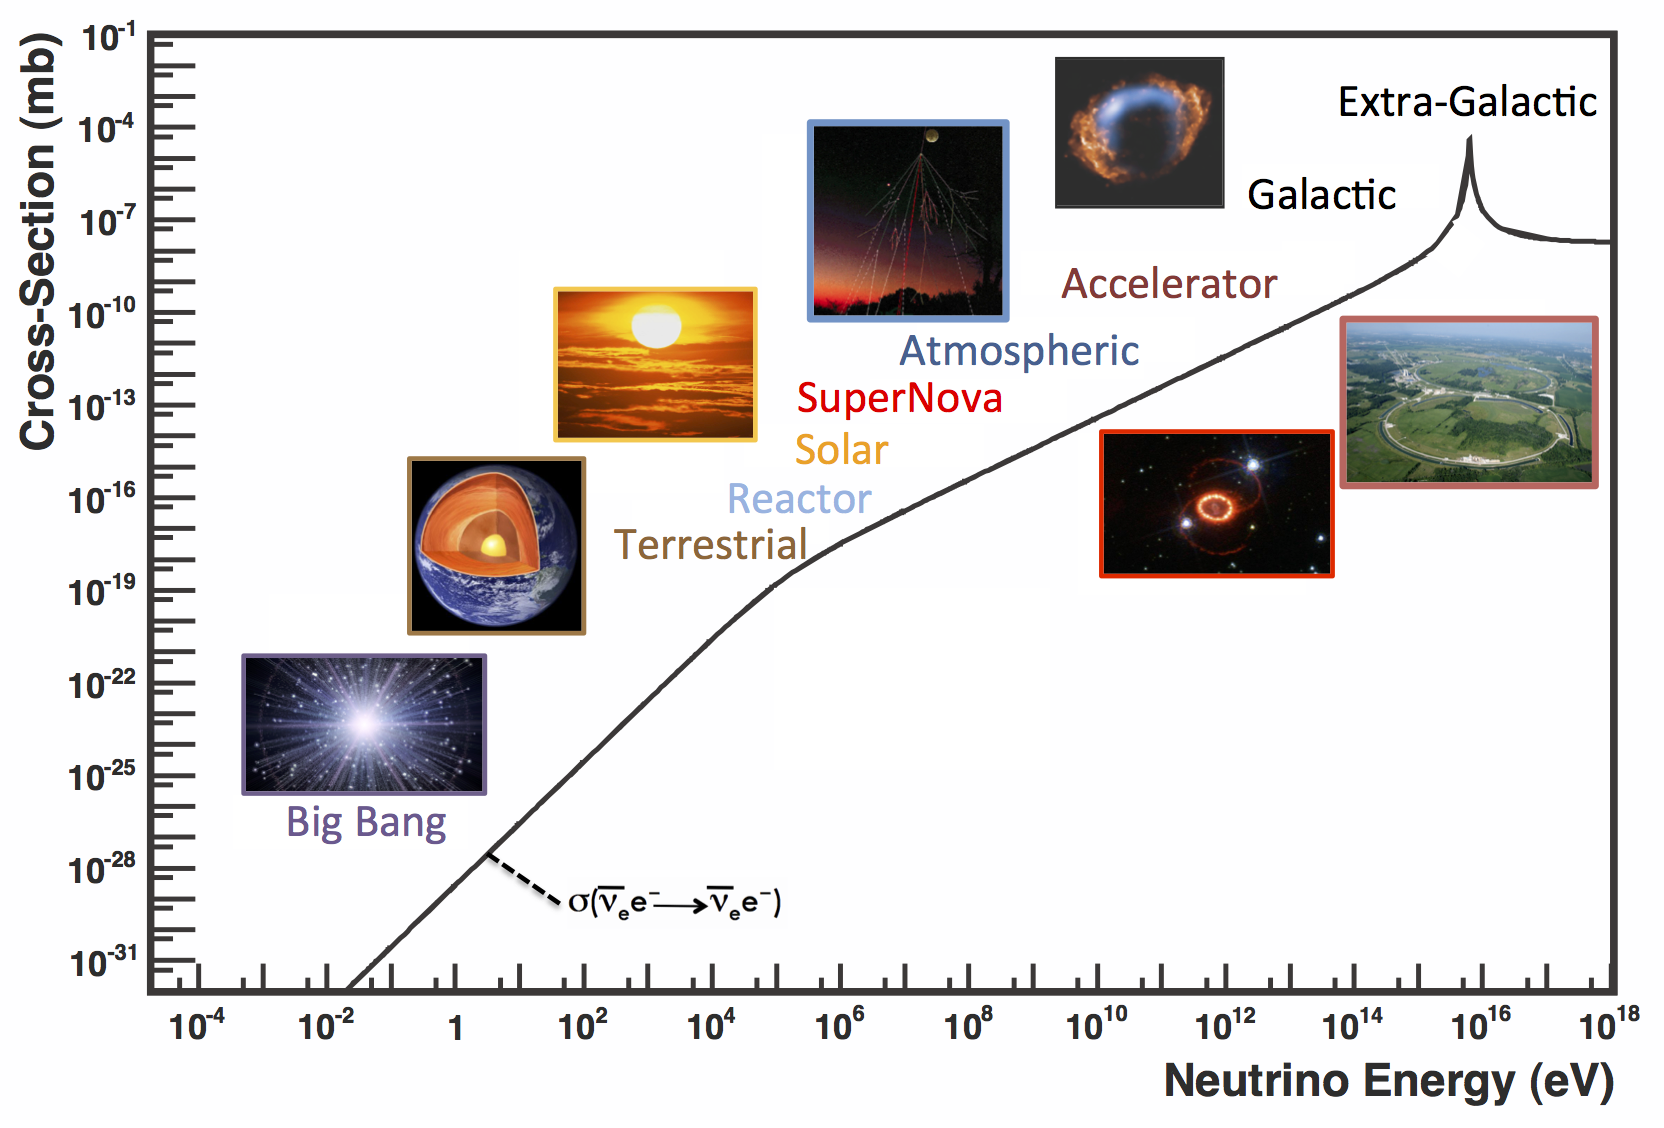
\includegraphics[scale=0.25]{img/NeutrinoSources.png}

Neutrinos are everywhere and we have produced and detected them by the millions. Eddington would not have made a living as a prophet (who does?)


%\end{block}
\end{columns}




\end{frame}



\section{Through the looking glass}
%\begin{frame}
\frametitle{Neutrinos through the looking glass}

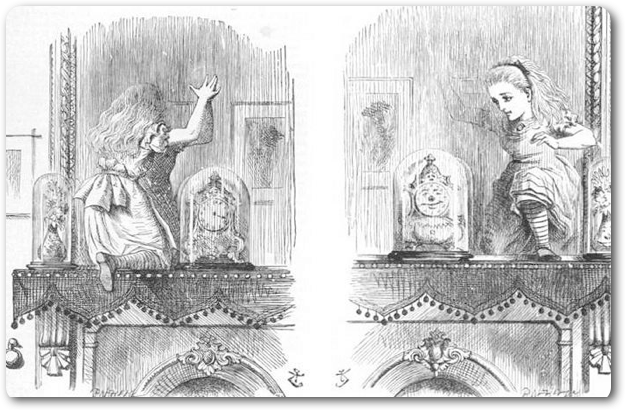
\includegraphics[scale=0.4]{img/Alice.png}

\end{frame}


\begin{frame}
\frametitle{Parity}
\begin{columns}
\column{0.5\textwidth}

\includegraphics[scale=0.45]{img/ParityCartoon.png}


The parity transformation changes a right-handed coordinate system into a left-handed one or vice versa. Two applications of the parity transformation restores the coordinate system to its original state.

It is a reasonable presupposition that nature should not care whether its coordinate system is right-handed or left-handed, \alert{but surprisingly, that turns out not to be so.}

\column{0.5\textwidth}
%\begin{block}{}
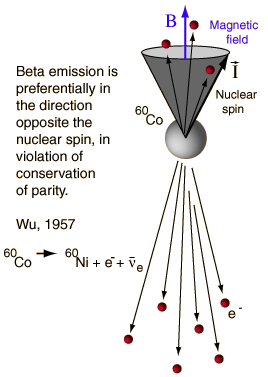
\includegraphics[scale=0.35]{img/wu.png}

In 1956, T. D. Lee and C. N. Yang predicted the non conservation of parity in the weak interaction. Their prediction was quickly tested when C. S. Wu and collaborators studied the beta decay of Cobalt-60 in 1957.

%\end{block}
\end{columns}

\end{frame}

%\begin{frame}
%\includegraphics[scale=0.35]{Cobalt.png}
%%wu.png
%\end{frame}
%GoldhaberExperiment.png
\begin{frame}
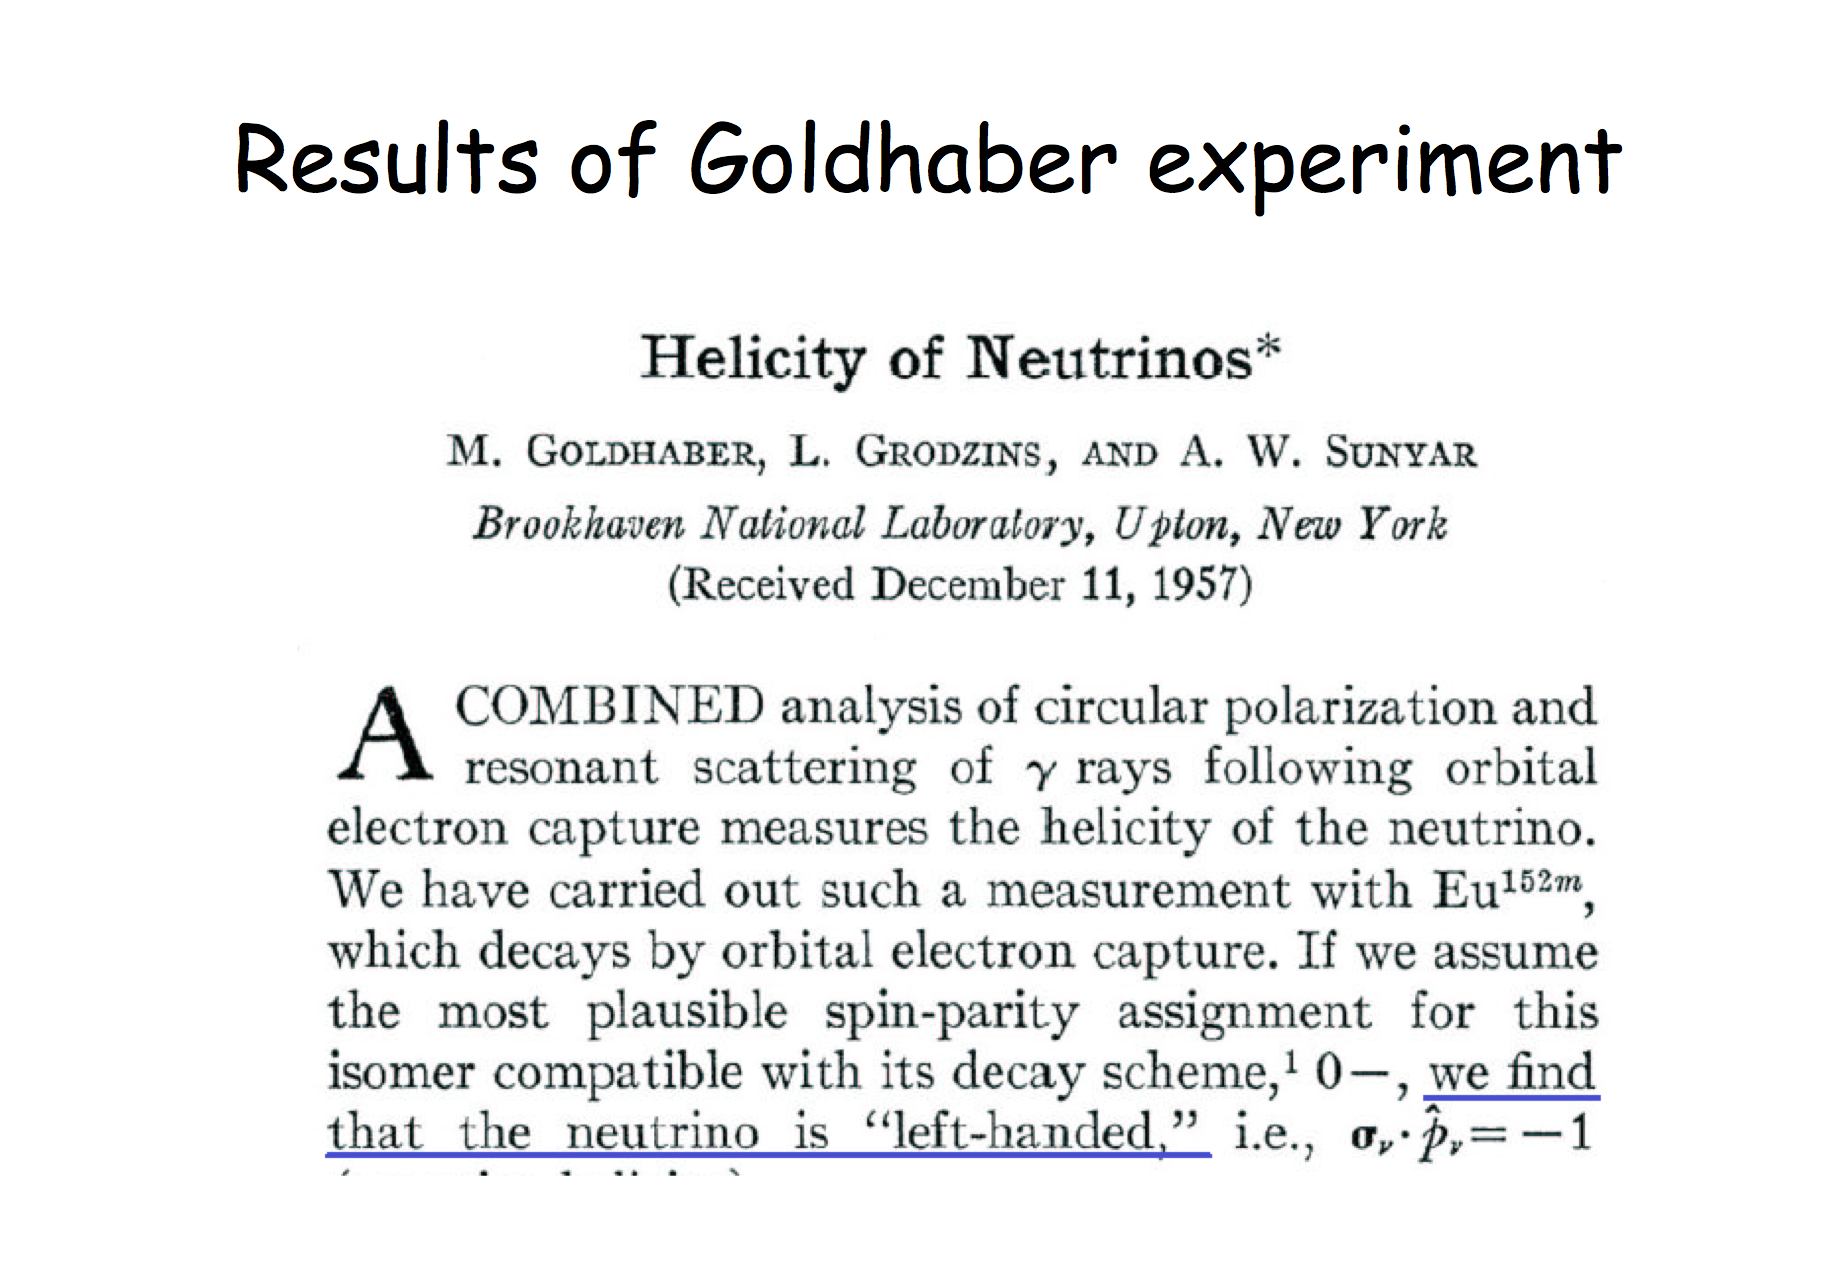
\includegraphics[scale=0.35]{img/Goldhaber.png}

\end{frame}

\begin{frame}
\frametitle{What do we talk about when we talk about helicity?}
\begin{columns}
\column{0.5\textwidth}
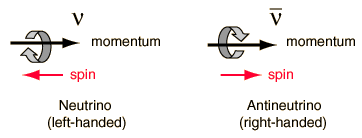
\includegraphics[scale=0.35]{img/NeutrinoHelicity.png}

Helicity is the spin projection in the direction of motion.
\[
h = \frac{\va{\sigma}\cdot \va{p}}{p}
\]
The Goldhaber experiment measured that neutrinos are left handed (spin opposed to motion, $h=-1$). The CPT theorem ensures that anti-neutrinos must be right-handed (spin along motion, $h=+1$).
\column{0.5\textwidth}

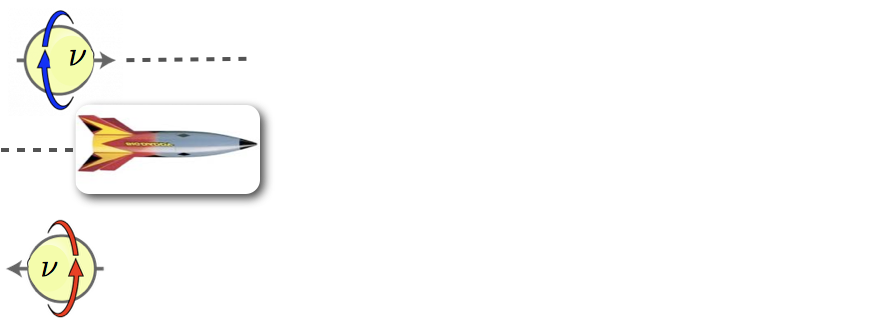
\includegraphics[scale=0.30]{img/neutrinoBoost2.png}

For massive particles, helicity depends on the reference frame and thus is not Lorentz invariant. One can always jump into a reference system faster than that of the particle and see its helicity flip.

But massless particles travel at the speed of light and cannot be overtaken. The helicity becomes a constant of motion. 
\end{columns}

\end{frame}

%
%\begin{frame}
%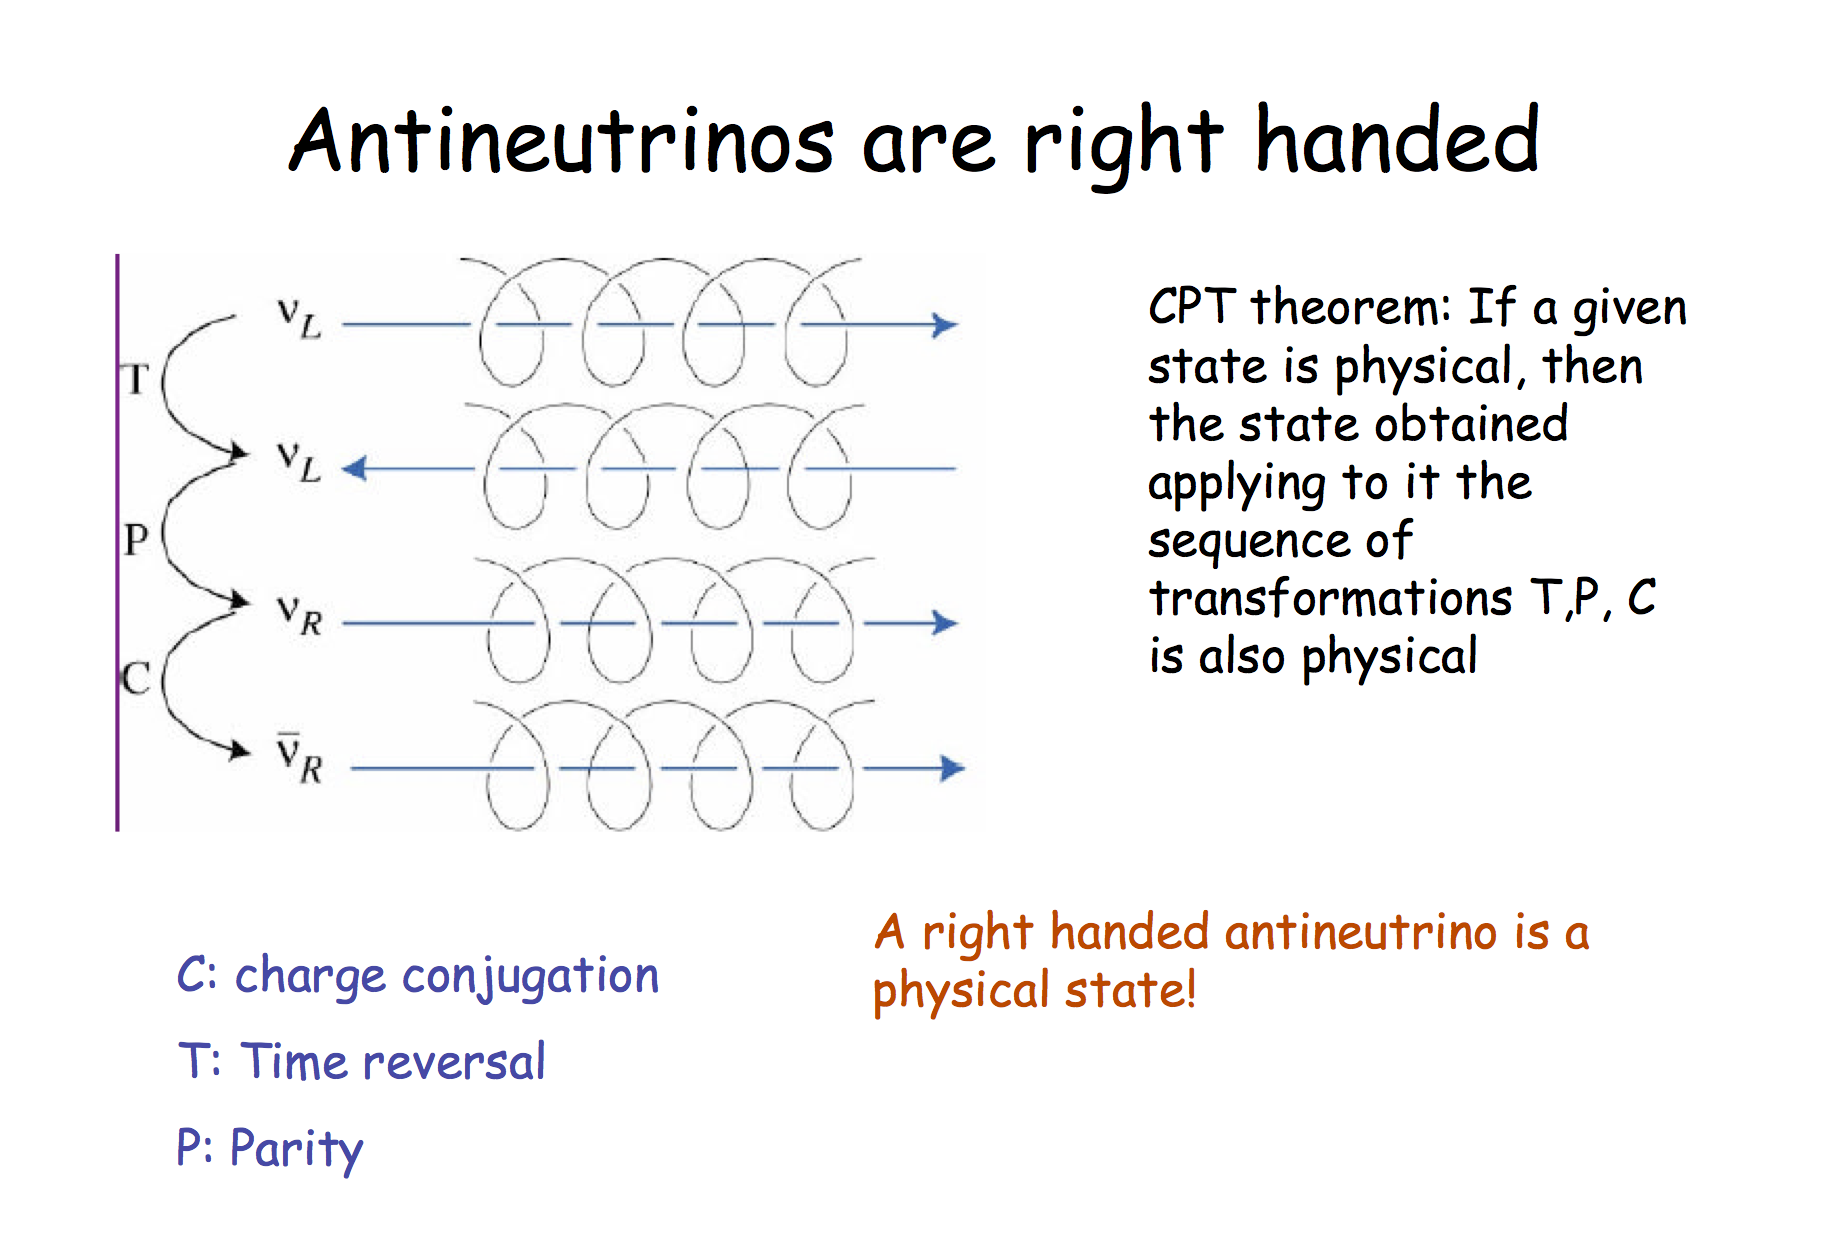
\includegraphics[scale=0.35]{AntineutrinosRH.png}
%
%\end{frame}

%\begin{frame}
%\frametitle{What do we talk about when we talk about (Standard Model) neutrinos?}
%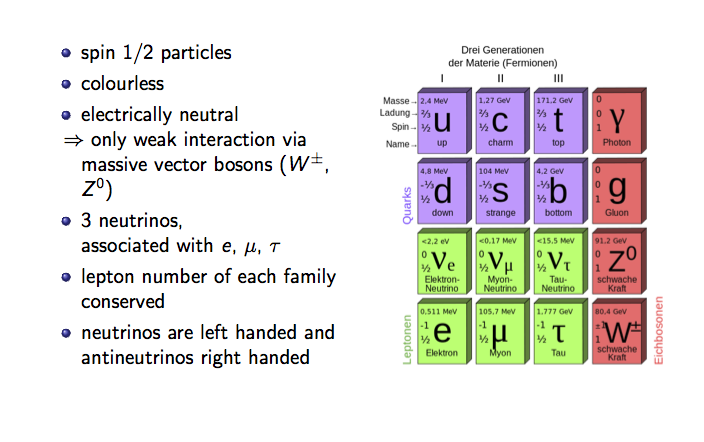
\includegraphics[scale=0.90]{NeutrinoOverview.png}
%\end{frame}

\begin{frame}
\frametitle{Neutrinos through the looking glass}
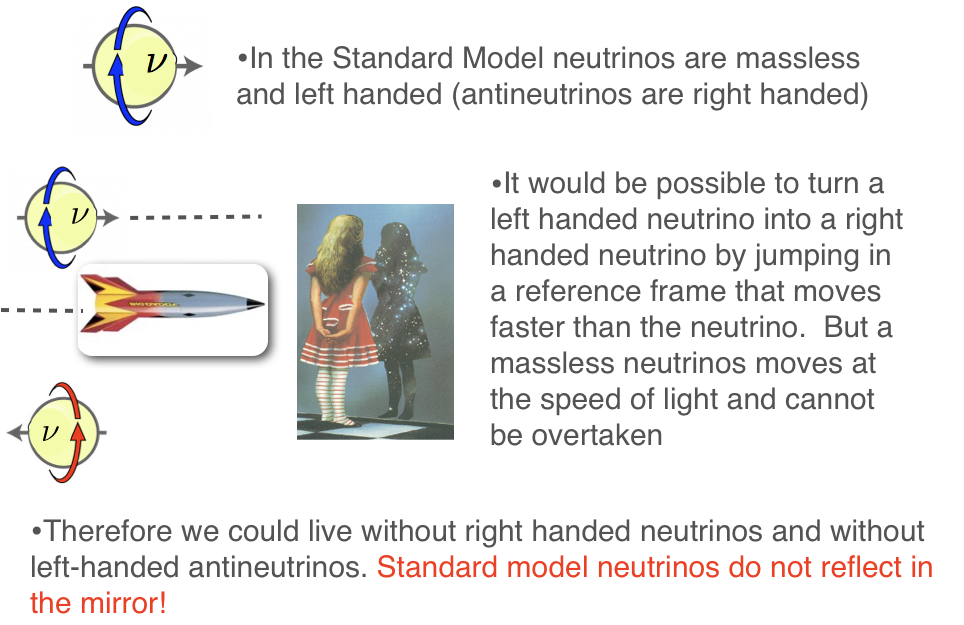
\includegraphics[scale=0.33]{img/NeutrinosLookingG.png}
\end{frame}

\begin{frame}
\frametitle{But what if neutrinos are massive}
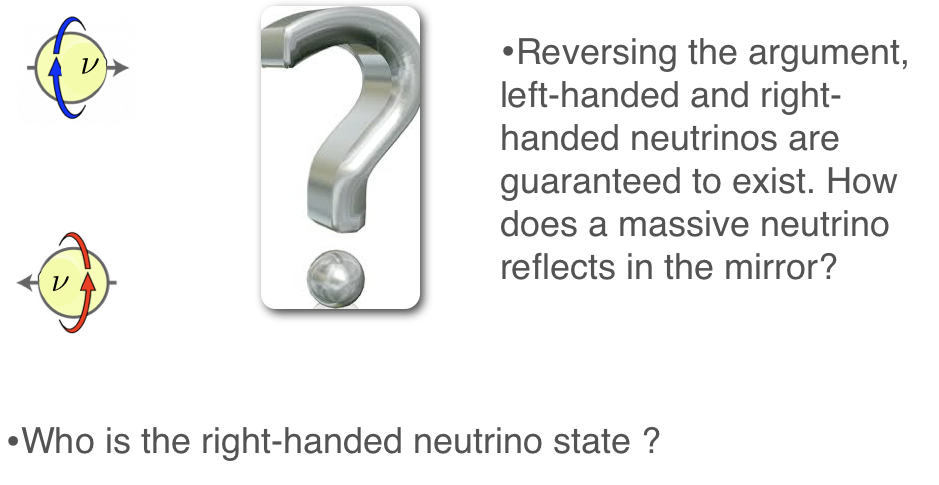
\includegraphics[scale=0.33]{img/WhatIfNeutrinoMassive.png}

\end{frame}






\section{Massive neutrinos}
%\begin{frame}
%\frametitle{Massless particles and helicity}
%\begin{columns}
%\column{0.5\textwidth}
%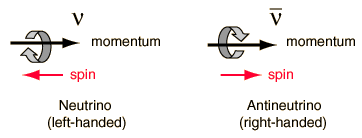
\includegraphics[scale=0.35]{img/NeutrinoHelicity.png}
%
%Helicity is the spin projection in the direction of motion.
%\[
%h = \frac{\va{\sigma}\cdot \va{p}}{p}
%\]
%In the limit of $m \rightarrow 0$~ Dirac's equation(s) decouple in 
%two states with definite helicity:
% \begin{empheq}[box=\fbox]{align}
%(E +  \va{p}\cdot\va{\sigma}) \chi  & = 0 \nonumber \\
%(E -  \va{p}\cdot\va{\sigma}) \phi  & = 0 \nonumber
%\end{empheq}
%The particle has negative helicity and the antiparticle positive helicity. \alert{Massless particles have well defined helicity}. \column{0.5\textwidth}
%
%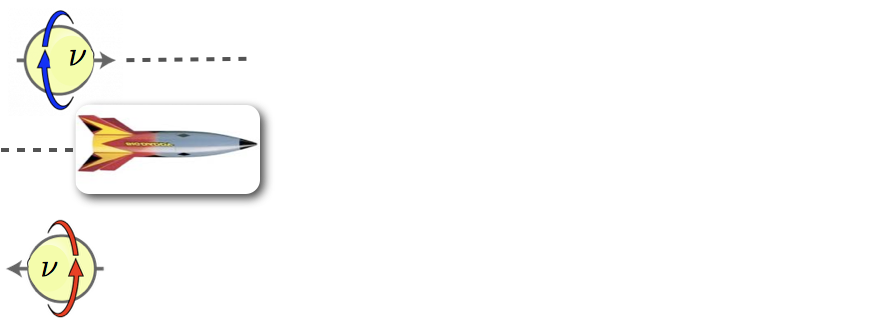
\includegraphics[scale=0.30]{img/neutrinoBoost2.png}
%
%For massive particles, helicity depends on the reference frame. One can always jump into a reference system faster than that of the particle and see its helicity flip.
%
%But massless particles travel at the speed of light and cannot be overtaken. The helicity becomes a constant of motion. 
%\end{columns}
%
%\end{frame}
%
%\begin{frame}
%\frametitle{Neutrino oscillations}
%%\begin{columns}
%%\column{0.4\textwidth}
%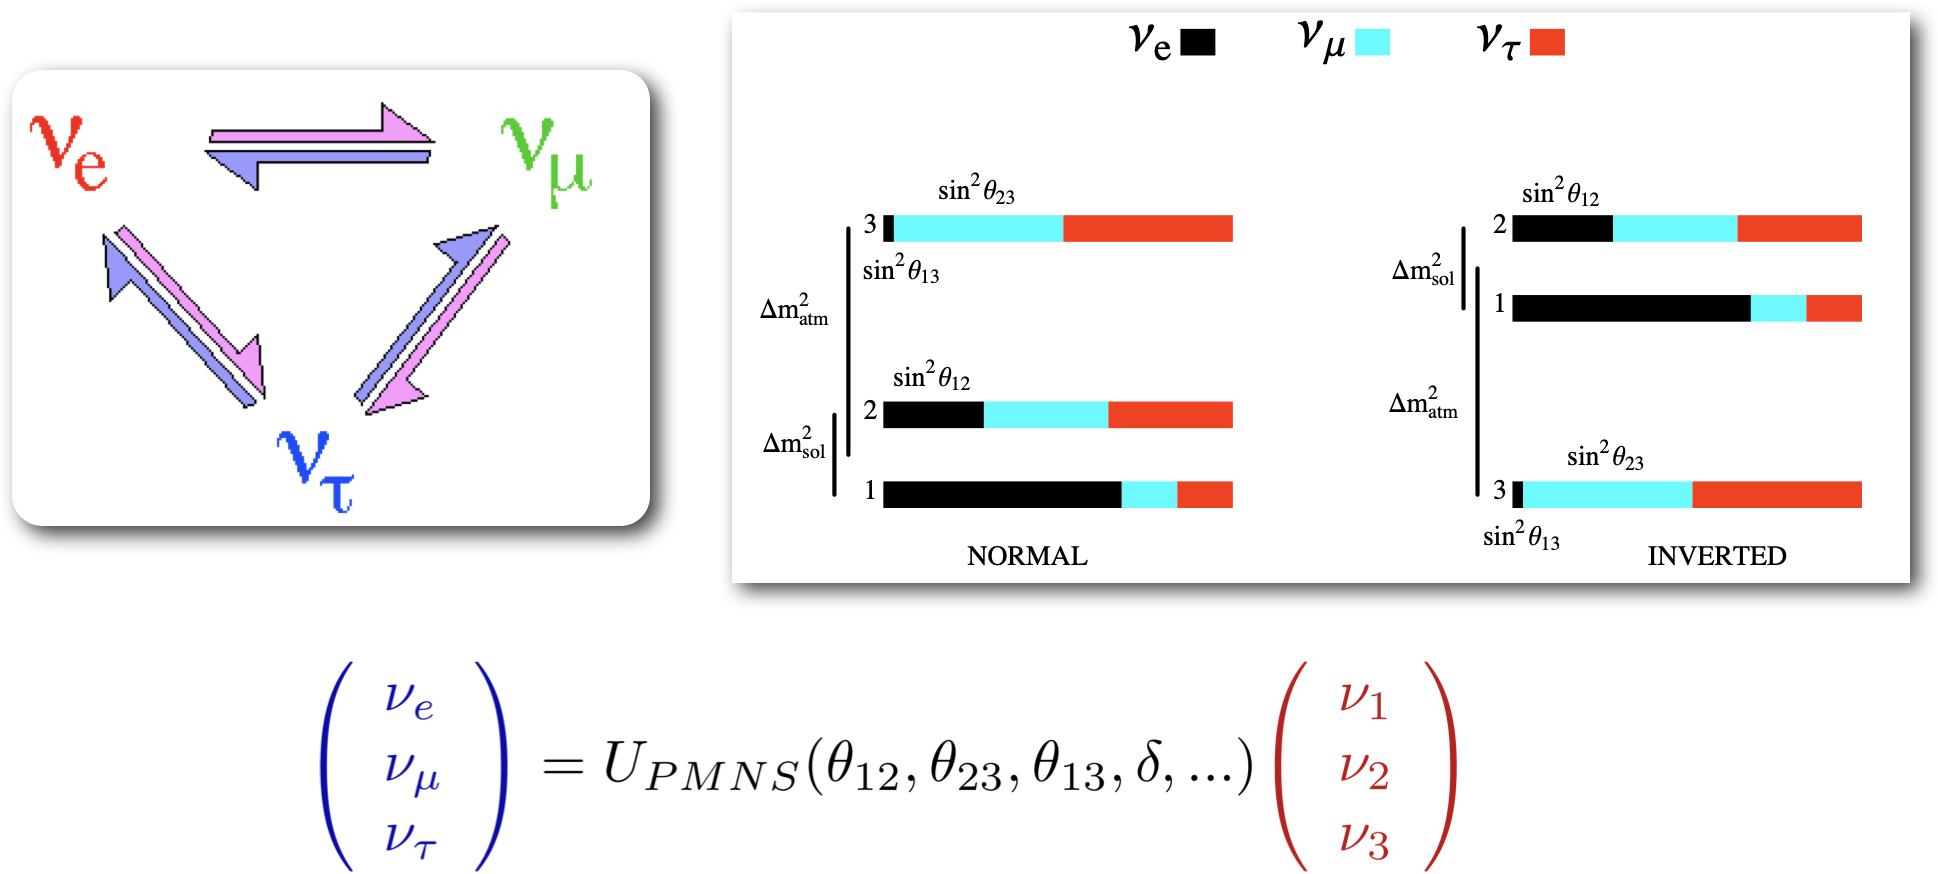
\includegraphics[scale=0.30]{img/neutrinoOscillations.png}
%%\column{0.4\textwidth}
%%\begin{block}{}
%
%Neutrino oscillation experiments (a story to be told some other time) have established that neutrinos are massive. Their mass is, however, very small. This is the reason why parity experiments found the neutrino to be left handed, since the effects associated to their masses are of the order of $m/E$~where $m$~is the mass of the neutrino (tiny) and $E$~the energy of the process (much larger). 
%
%\alert{But how do we give a mass to the neutrinos?} 
%
%%\end{block}
%%\end{columns}
%\end{frame}
%
%\begin{frame}
%\frametitle{Electron mass}
%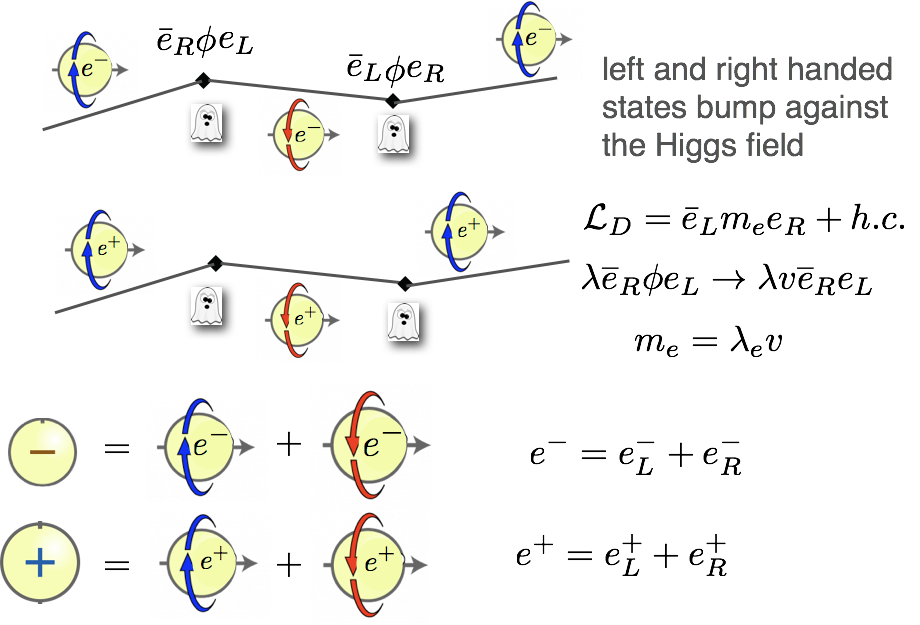
\includegraphics[scale=0.30]{img/ElectronMass.png}
%\end{frame}

\begin{frame}
\frametitle{Neutrino mass (Dirac recipe)}
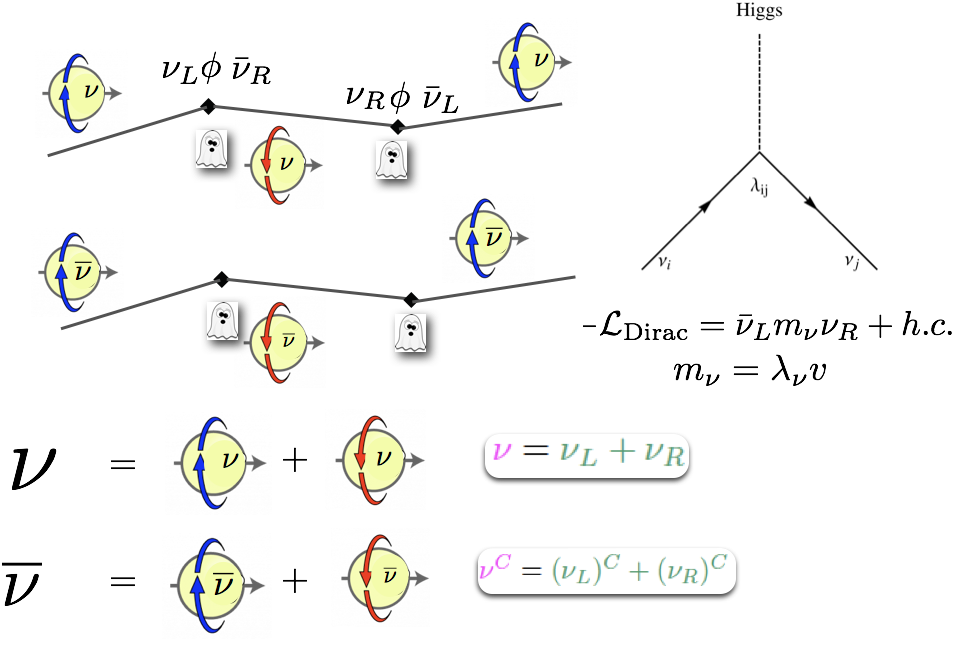
\includegraphics[scale=0.30]{img/NeutrinoMassDirac.png}
\end{frame}

\begin{frame}
\frametitle{Deus ex machina}
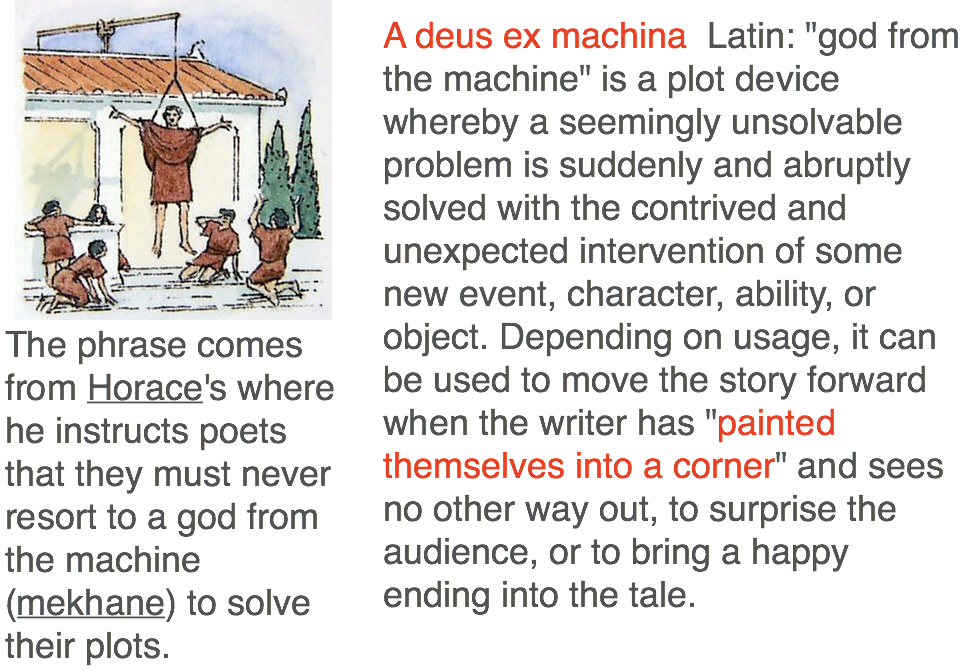
\includegraphics[scale=0.30]{img/DeusExMachina.png}
\end{frame}

\begin{frame}
\frametitle{Dirac neutrino mass: Deus ex machina}
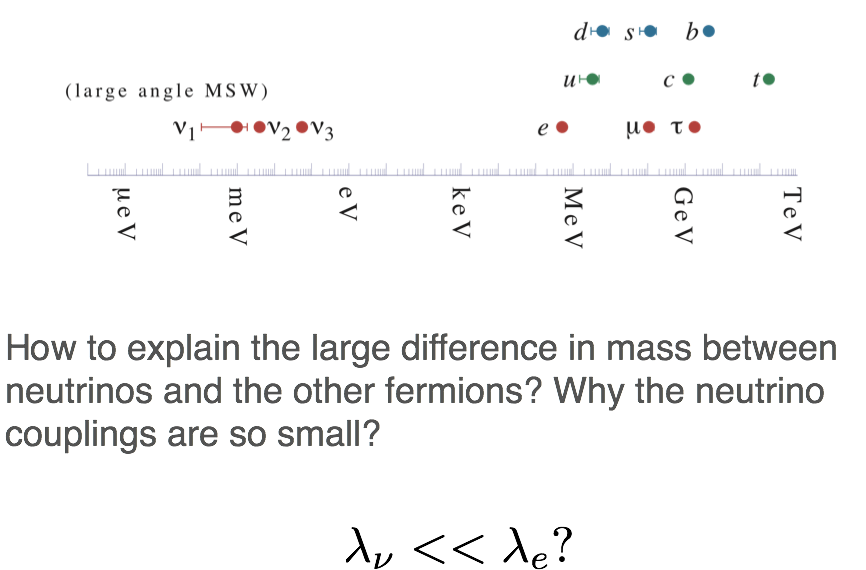
\includegraphics[scale=0.30]{img/SmallNeutrinoMasses.png}
\end{frame}

\begin{frame}
\frametitle{Majorana neutrinos}
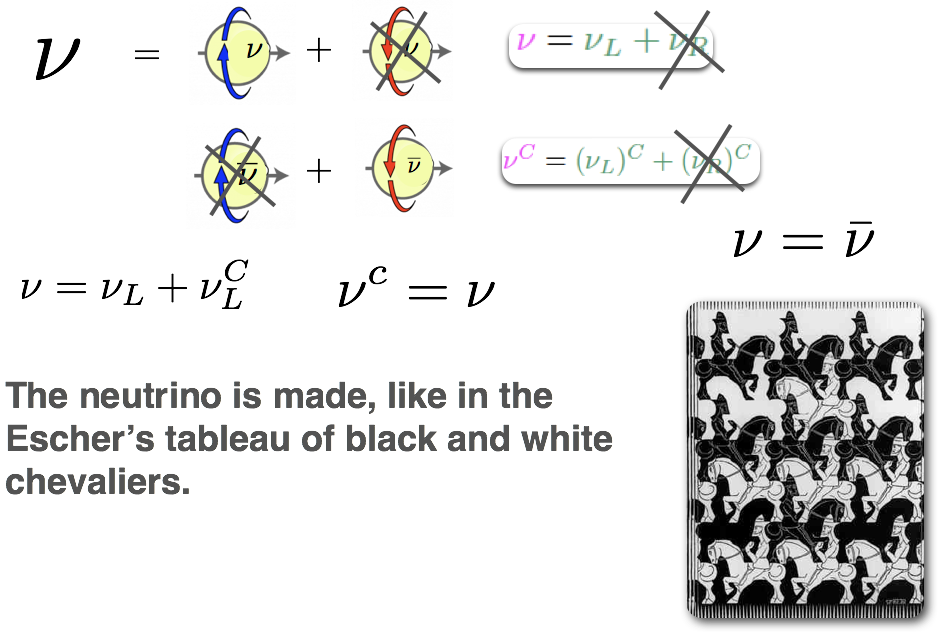
\includegraphics[scale=0.30]{img/MajoranaNeutrinosCartoon.png}
\end{frame}

\begin{frame}
\frametitle{Majorana mass}
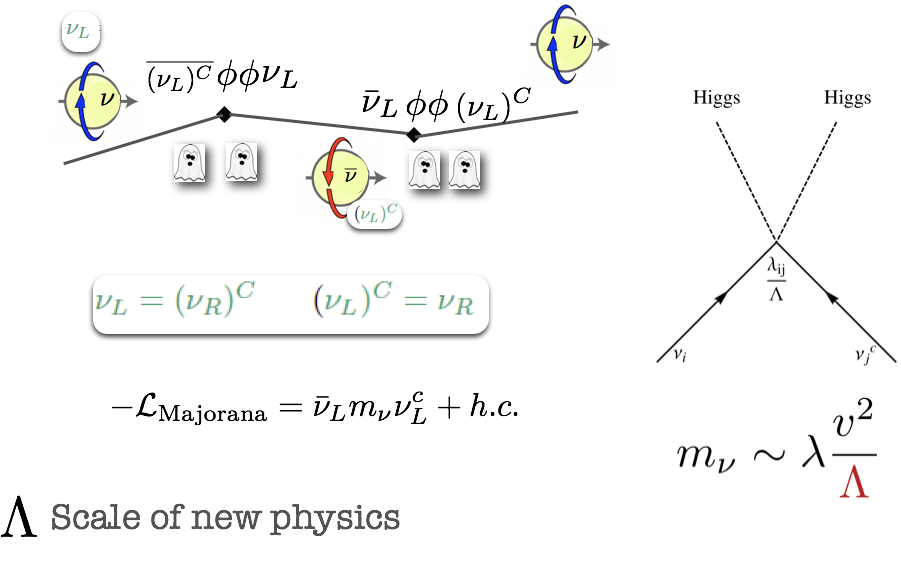
\includegraphics[scale=0.30]{img/MajoranaMass.png}
\end{frame}

\begin{frame}
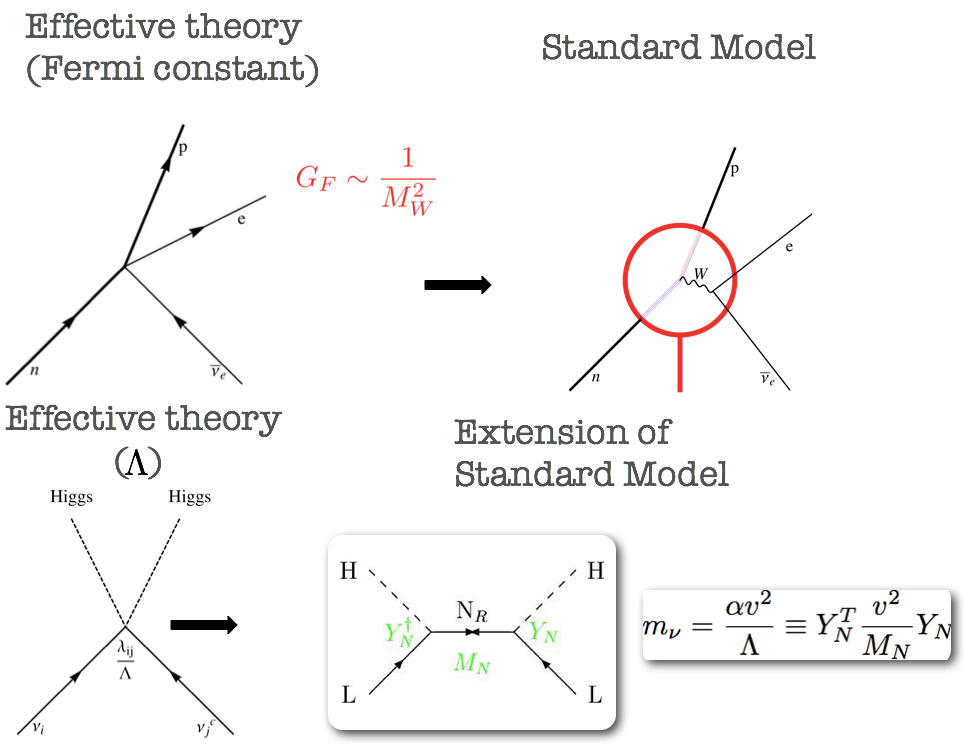
\includegraphics[scale=0.30]{img/Effective.png}
\end{frame}

\begin{frame}
\frametitle{The mystery of the missing antimatter}
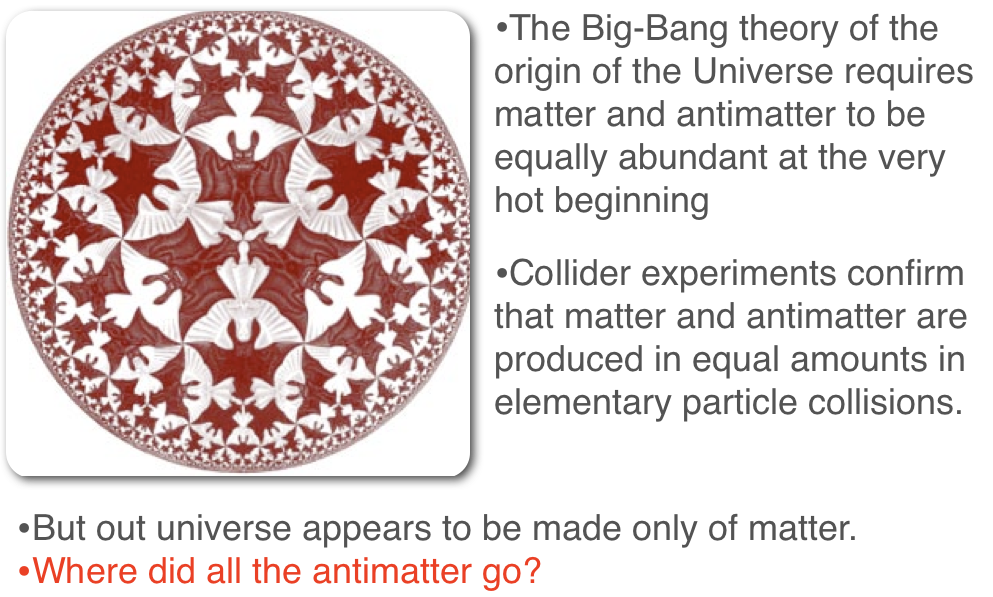
\includegraphics[scale=0.30]{img/MissingAntiMatter.png}
\end{frame}

\begin{frame}
\frametitle{CP violation and Majorana neutrinos}
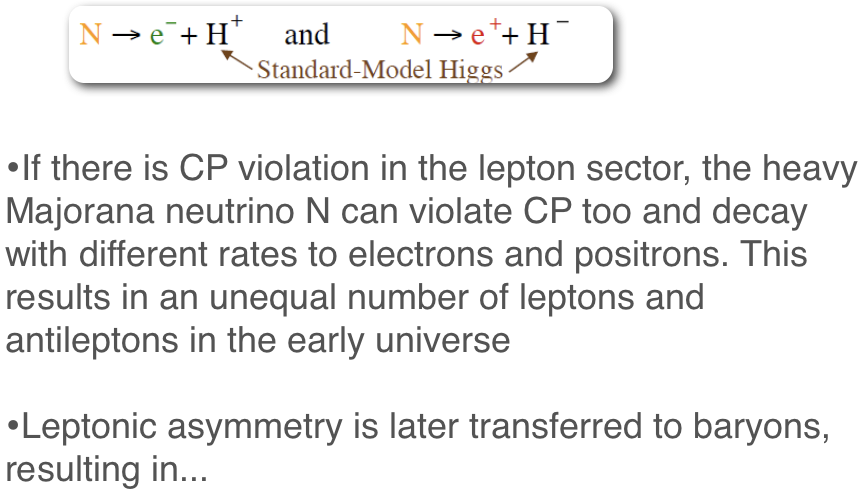
\includegraphics[scale=0.30]{img/CP.png}
\end{frame}

\begin{frame}
\frametitle{We are the leftovers}
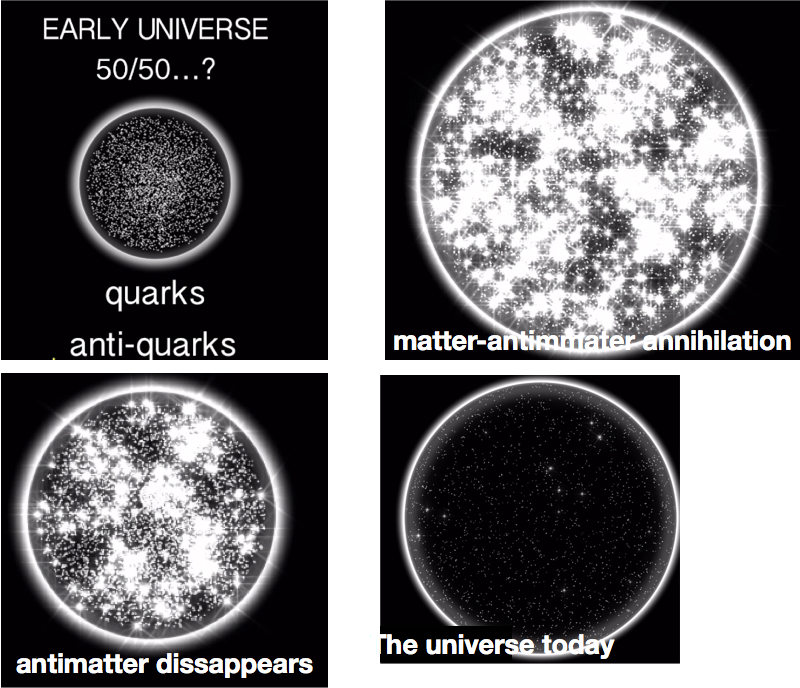
\includegraphics[scale=0.30]{img/MissingUniverse.png}
\end{frame}
%

\begin{frame}
\frametitle{A formula for the Universe}
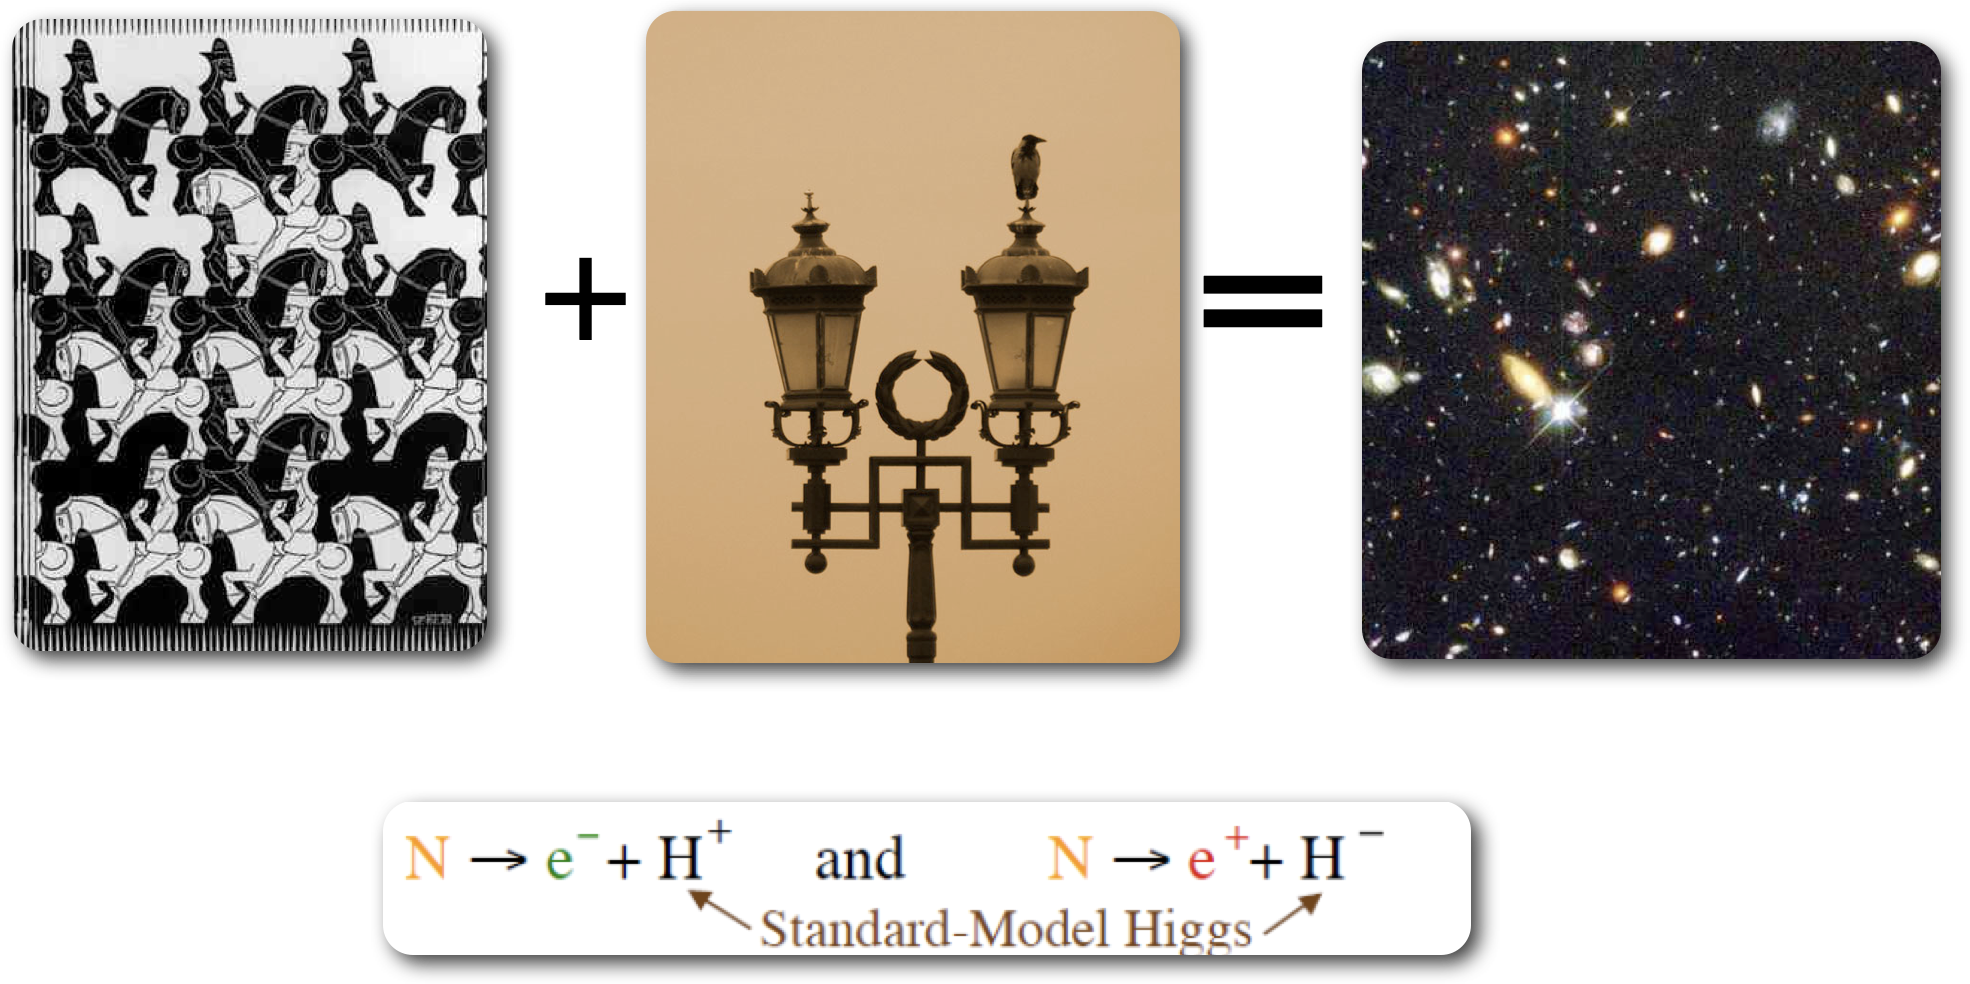
\includegraphics[scale=0.30]{img/formulaUniverse.png}
\end{frame}











%\begin{frame}
\frametitle{What do we talk about when we talk about Dirac?}
\begin{columns}
\column{0.35\textwidth}
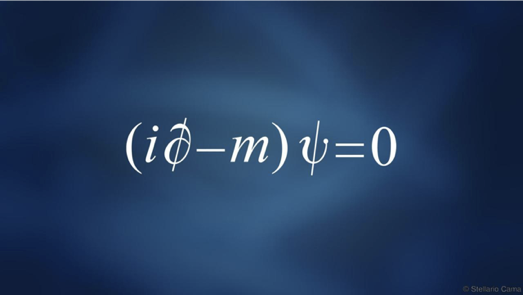
\includegraphics[scale=0.20]{img/dirac-eq.png}
 
 \column{0.6\textwidth}
%\begin{block}{}
If neutrinos were fermions of spin 1/2 they could presumably described by Dirac equation. Dirac had proposed his famous equation in 1928, two years before the neutrino was proposed by Pauli.  In 1929 P.A.M. Dirac had published his famous paper predicting antimatter (the positron), who would be discovered shortly after by Andersen. Yet, in 1930, antimatter was a concept as fantastic and hard to believe in as the neutrino itself.  

%\end{block}
\end{columns}
\end{frame}

\begin{frame}
\frametitle{The quantum theory of the electron}

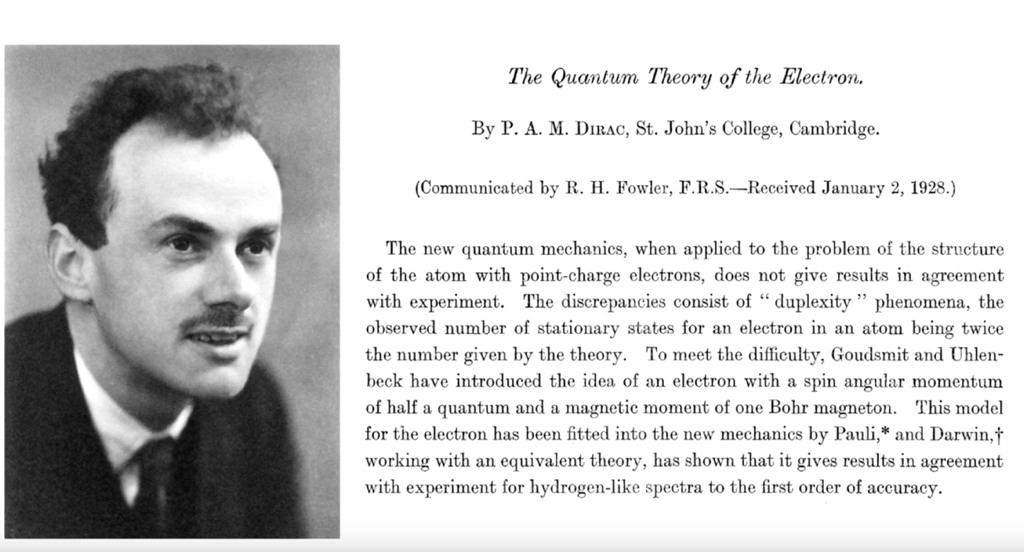
\includegraphics[scale=0.3]{img/dirac-eq-paper.png}
 
\end{frame}

\begin{frame}
\frametitle{The Klein Gordon equation}
The Dirac equation describes spin-1/2 particles such electrons and neutrinos. It emerges from Dirac's attempt to avoid the negative solutions in the equation of Klein-Gordon which is obtained when one quantizes the relativistic relation:
\[
E^2 = p^2 + m^2 \, \, {(\rm with~ c = 1)}
\]
through the quantum-mechanical recipe:
\[
E \rightarrow i \frac{\partial}{\partial_t}, \,\, \vv{\bm{P}} \rightarrow -i \vv{\bm{\nabla}}
\]
then we obtain the Klein Gordon equation


\begin{empheq}[box=\fbox]{align}
   (i \frac{\partial}{\partial_t})^2 \psi= [(-i \bar{\nabla})^2 + m^2] \psi \nonumber
\end{empheq}

%\[
%(i \frac{\partial}{\partial_t})^2 \psi= [(-i \bar{\nabla})^2 + m^2] \psi
%\]
%which is the KG equation. 

The wavefunction $\psi$~ is now a relativistic scalar and the space and time derivatives are both
second order. However, the initial values of $\psi$~  and
$\partial \psi$~  can be chosen freely, and as a result the probability density is no longer positive definite. 
This leaves open the possibility of negative probabilities.
\end{frame}

\begin{frame}
\frametitle{Linearizing $E = \sqrt{p^2 + m^2}$}
Dirac approach was to attempt linearizing the relativistic energy-momentum equation
\[
E = \sqrt{p^2 + m^2} = \vv{\bm{\alpha}}\cdot \vv{\bm{P}} + \beta \cdot m = 
\alpha_x p_x + \alpha_y p_y + \alpha_z p_z + \beta m
\]
Squaring both sides:

\begin{align*}
E^2 = p^2 + m^2 = & (\alpha_x p_x + \alpha_y p_y + \alpha_z p_z + \beta m) 
(\alpha_x p_x + \alpha_y p_y + \alpha_z p_z + \beta m) \\
%= & \alpha_x^2 p_x^2 + \alpha_y^2 p_y^2 + \alpha_z^2 p_z^2 + \beta^2 m^2 \\
%+ & (\alpha_x \alpha_y + \alpha_y \alpha_x) p_x p_y \\
%+ & (\alpha_x \alpha_z + \alpha_z \alpha_x) p_x p_z \\
%+ & (\alpha_y \alpha_z + \alpha_y \alpha_y) p_y p_z \\
%+ & (\alpha_x \beta + \beta \alpha_x) m p_x \\
%+ & (\alpha_y \beta + \beta \alpha_y) m p_y \\
%+ & (\alpha_z \beta + \beta \alpha_z) m p_z \\
= & p_x^2 + p_y^2 + p_z^2 + m^2
%
\end{align*}
The above equation can only be solved if the $\alpha_i, \beta$~are matrices of at least rank 4, which satisfy:
 \begin{empheq}[box=\fbox]{align}
  \{\alpha_i, \alpha_j\}&=0 \, \, ( i \neq j)\\ 
\{\alpha_i, \beta\} & = 0 \nonumber
\end{empheq}
where:
\[
\{A, B\} = AB + BA
\]
\end{frame}

\begin{frame}
\frametitle{Constructing $\bf{\alpha}$~and $\bf{\beta}$~using Pauli matrices }
%\begin{block}{}
%Since the $\alpha, \beta$~do not commute, they cannot be numbers. \alert{They need to be matrices}. In fact, they are traceless hermitian ($A^\dagger = A$) matrices or rank greater or equal than four. 
%\end{block}

They $\alpha, \beta$ can be constructed in terms of the  Pauli matrices:
\[
\alpha_i = 
\begin{pmatrix} 
0 & \sigma_i \\
\sigma_i & 0 
\end{pmatrix} \, \, ,
\beta = 
\begin{pmatrix} 
I & 0 \\
0 & -I 
\end{pmatrix} 
\]

where $I$~is the $2 \times 2$~ identity matrix, and the Pauli matrices are:
\[
\sigma_1 = 
\begin{pmatrix} 
0 & 1 \\
1& 0 
\end{pmatrix} \, \, ,
\sigma_2 = 
\begin{pmatrix} 
0 & -i \\
i & 0 \\ 
\end{pmatrix} \, \, ,
\sigma_3 = 
\begin{pmatrix} 
1 & 0 \\
0 & -1 \\ 
\end{pmatrix}
\]

Pauli matrices exhibit clearly the properties of being hermitian and traceless,
$\sigma_i^\dagger = \sigma_i$, $Tr \sigma_i = 0$, and $\sigma_i^2 = I$. They satisfy the commutation relations: 
\begin{empheq}[box=\fbox]{align}
 %\begin{empheq}[box=\tcbhighmath]{align}
\{\sigma_i, \sigma_j\}&=2 \delta_{ij} \, \, ( i,j,k = 1, 2, 3)\\
[\sigma_i, \sigma_j] & = 2 i \epsilon_{ijk} \sigma_k \nonumber
\end{empheq}
\end{frame}
\begin{frame}

\frametitle{The Dirac equation }
using the linearized equation
\[
E  -\va{\alpha}\cdot \va{P} - \beta \cdot m = 0
\]
and substituting operators
\[
E \rightarrow i \frac{\partial}{\partial_t}, \,\, \va{P} \rightarrow -i \va{\nabla}
\]
One obtains the Dirac equation
\[
 i \frac{\partial}{\partial_t} \psi = [ \va{\alpha} (-i\va{\nabla}) + \beta m] \psi
\]

Multiply now $\beta$~from the left and define  the gamma matrices:
\[
 \gamma^0 = \beta = \begin{pmatrix} 
I & 0 \\
0 & -I 
\end{pmatrix}  \,\,\, ,  \gamma^i = \beta \alpha_i = \begin{pmatrix} 
0 & \sigma_i \\
-\sigma_i & 0 
\end{pmatrix} 
\]
To obtain 
%
%\begin{empheq}[box=\fbox]{align}
%(E \gamma^0 -\va{p}\cdot \va{\gamma} -m ) \psi & = 0 \nonumber
%\end{empheq}
%\[
%[i(\gamma^0 \partial_0 + \gamma^i \partial_i) -m ] \psi  = 0
%\]
%or
 \begin{empheq}[box=\fbox]{align}
(i \gamma^\mu \partial_\mu -m ) \psi & = 0 \nonumber
\end{empheq}
%\end{frame}

The  $\gamma$~matrices are not unique. Any set that satisfy the anticommutation relations (Clifford algebra) can be used:
%
\begin{empheq}[box=\fbox]{align}
\{\gamma^\mu, \gamma^\nu\} = 2 g^{\mu\nu} \nonumber
\end{empheq}
\end{frame}

%\begin{frame}
%Alternatively, in terms of the energy and momentum operators:
%\begin{empheq}[box=\fbox]{align}
%(E \gamma^0 -\va{p}\cdot \va{\gamma} -m ) \psi & = 0 \nonumber
%\end{empheq}
%
%In this equation $\psi$~is the Dirac bispinor: 
%\[
%\psi = \mqty(\psi_1 \\ \psi_2 \\ \psi_3 \\ \psi_4) =  \mqty(\phi \\ \chi); \,\,\,
%\phi =  \mqty(\phi_1 \\ \phi_2), \,\,\, \chi =  \mqty(\chi_1 \\ \chi_2)
%\]
%The two spinors $\phi$~and $\chi$~represent the particle and the antiparticle; the two components of each of them represent the two states of the third component of the spin, $s_z = +1/2$~and
%$s_z = -1/2$.
%
%The four $\gamma$~matrices, found before, are not unique. Any set that satisfy the anticommutation relations (Clifford algebra) can be used:
%
%\begin{empheq}[box=\fbox]{align}
%\{\gamma^\mu, \gamma^\nu\} = 2 g^{\mu\nu} \nonumber
%\end{empheq}
%\end{frame}



%\begin{frame}
\frametitle{Plane wave solutions of the Dirac equation}
For a particle at rest, $\va{p} = 0$ and the Dirac equation becomes:
\[
i\gamma^0\partial_0\psi = m \psi, \,\,\, or \, \, \,  i \mqty(1 & 0 & 0 & 0\\ 0 & 1 & 0 & 0 \\
0 & 0 & -1 & 0 \\ 0 & 0 & 0 & -1 ) \ \mqty(\dot{\psi_1} \\ \dot{\psi_2}\\ \dot{\psi_3} \\ \dot{\psi_4}) = 
m \mqty(\psi_1 \\ \psi_2\\ \psi_3 \\ \psi_4)
\]
There are four independent solutions: two describe particle-antiparticle and two describe spin up-down
\[
\psi^{(1)} = w^{(1)} e^{-i m\cdot t}, \,\,\, \psi^{(2)} = w^{(2)} e^{-i m\cdot t}, \,\,\,
\psi^{(3)} = w^{(3)} e^{+i m\cdot t}, \,\,\, \psi^{(4)} = w^{(4)} e^{i m\cdot t}
\]
\[
w^{(1)} = \mqty(1 \\ 0 \\ 0 \\ 0), \,\,\, w^{(1)} = \mqty(0\\ 1 \\ 0 \\ 0), \,\,\,
w^{(3)} = \mqty(0 \\ 0 \\ 1 \\ 0), \,\,\, w^{(4)} = \mqty(0 \\ 0 \\ 0 \\ 1), \,\,\,
\]

\end{frame}
%\begin{frame}
%\frametitle{The solutions are eigenvalues of the spin}
%The solutions are eigenvalues of the z-component of the spin, $\Sigma_3$, which in the Dirac representation is:
%\[
%\Sigma_3 = \mqty(\sigma_3 & 0 \\ 0 &  \sigma_3) = \mqty(1 & 0 & 0 & 0\\ 0 & -1 & 0 & 0 \\
%0 & 0 & 1 & 0 \\ 0 & 0 & 0 & -1 )
%\]
%thus:
%\[
%\psi^{(1)} : \Sigma_3 = +1, \,\,\,
%\psi^{(2)} : \Sigma_3 = -1, \,\,\,
%\psi^{(3)} : \Sigma_3 = +1, \,\,\,
%\psi^{(4)} : \Sigma_3 = -1.
%\]
%\end{frame}
%
\begin{frame}
\frametitle{Negative energy solutions}

Since we define the eigenvalue of the operator $\pdv{t}$~to be the energy, we find that 
$\psi^{(1)}$~and $\psi^{(2)}$~are positive energy solutions and 
$\psi^{(3)}$~and $\psi^{(4)}$~are negative energy solutions.

\begin{alertblock}{Surprise!}
Dirac's equation \alert{predicts} negative energy solutions.
\end{alertblock}
\end{frame}

\begin{frame}
\frametitle{Dirac struggle with negative energy solutions: protons}

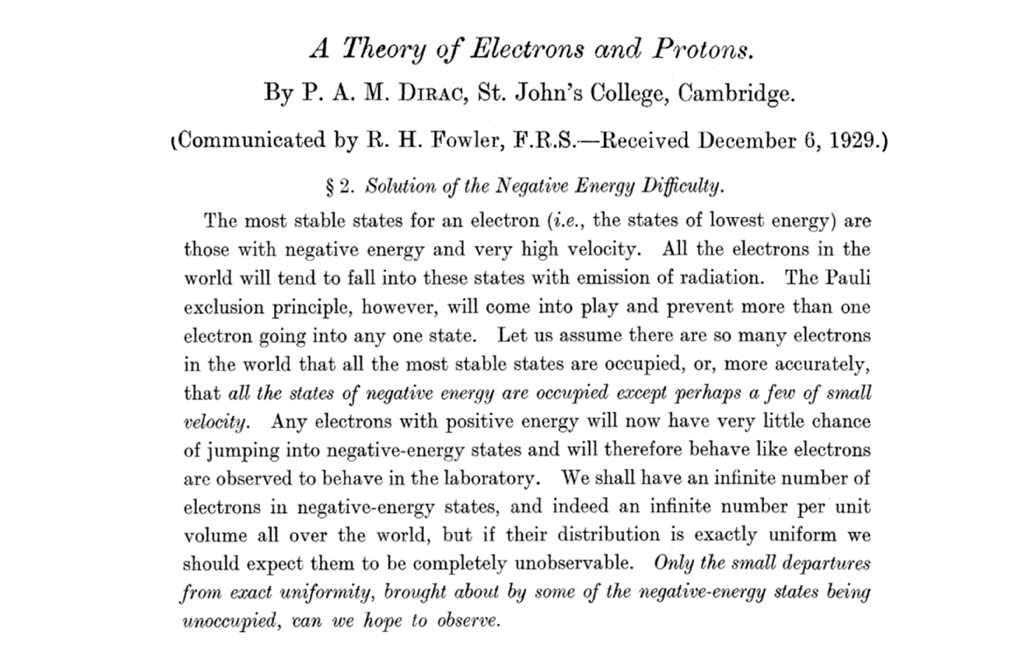
\includegraphics[scale=0.3]{img/DiracElectronProton.png}
\end{frame}

\begin{frame}
\frametitle{The opinion of Heisemberg}

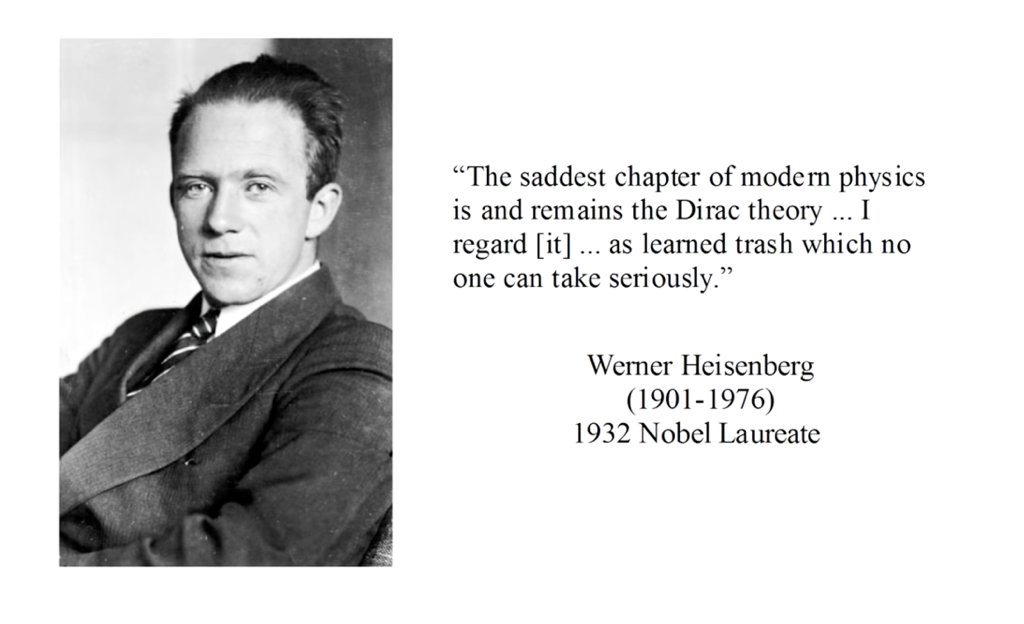
\includegraphics[scale=0.3]{img/HeisembergOpinionDirac.png}
\end{frame}

\begin{frame}
\frametitle{Identifying holes in the negative sea with positrons}

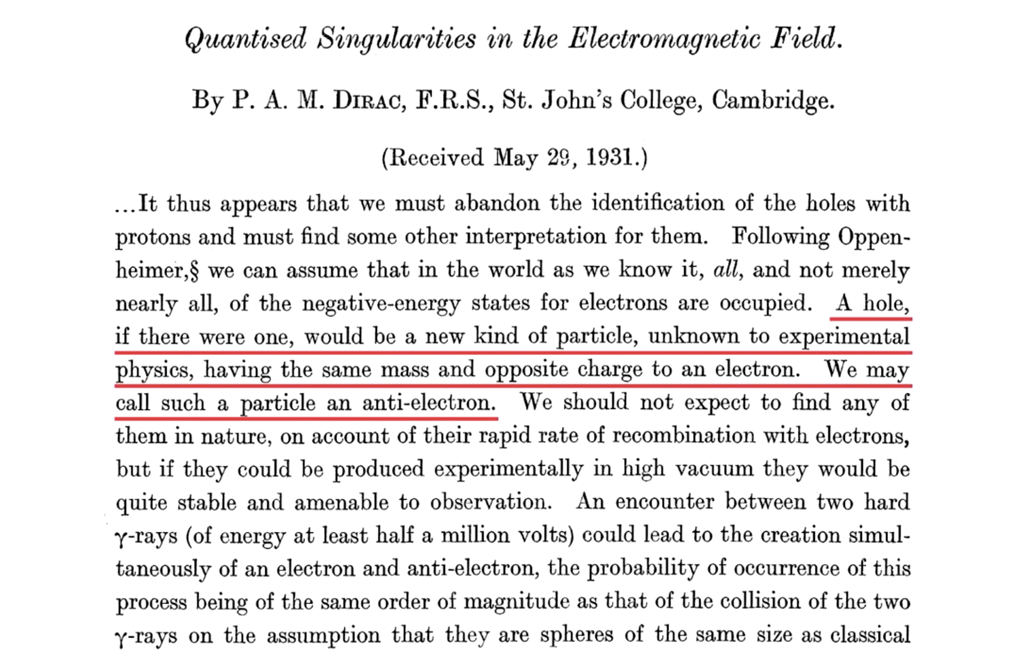
\includegraphics[scale=0.3]{img/diracPositrons.png}
\end{frame}

\begin{frame}
\frametitle{The discovery of the positron (Andersen, 1932)}

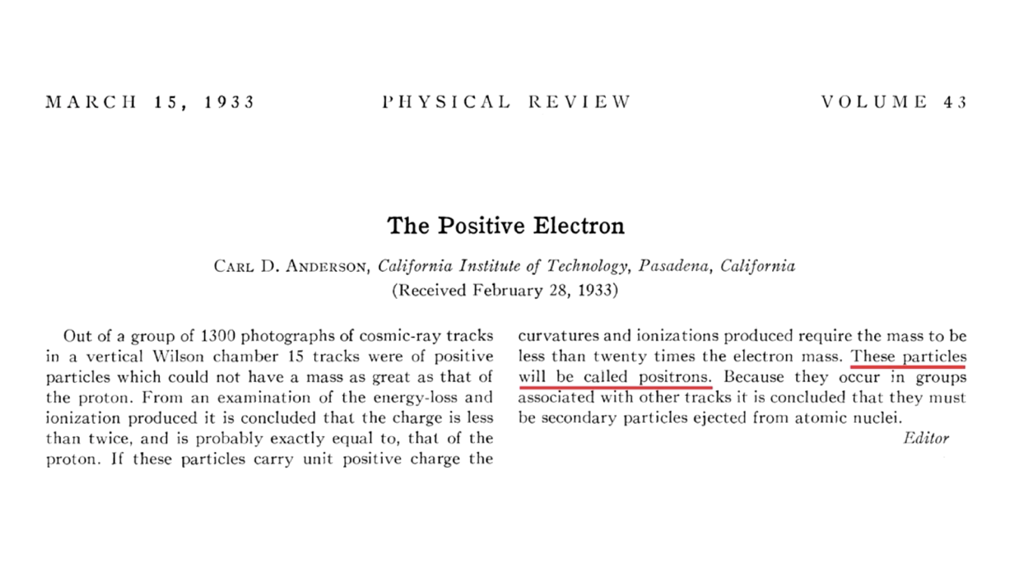
\includegraphics[scale=0.3]{img/AndersonPaper.png}
\end{frame}

%\begin{frame}
%\frametitle{The positron is real}
%
%\includegraphics[scale=0.3]{positronDiscovery.png}
%\end{frame}
%

\begin{frame}
\frametitle{The negative sea parable}

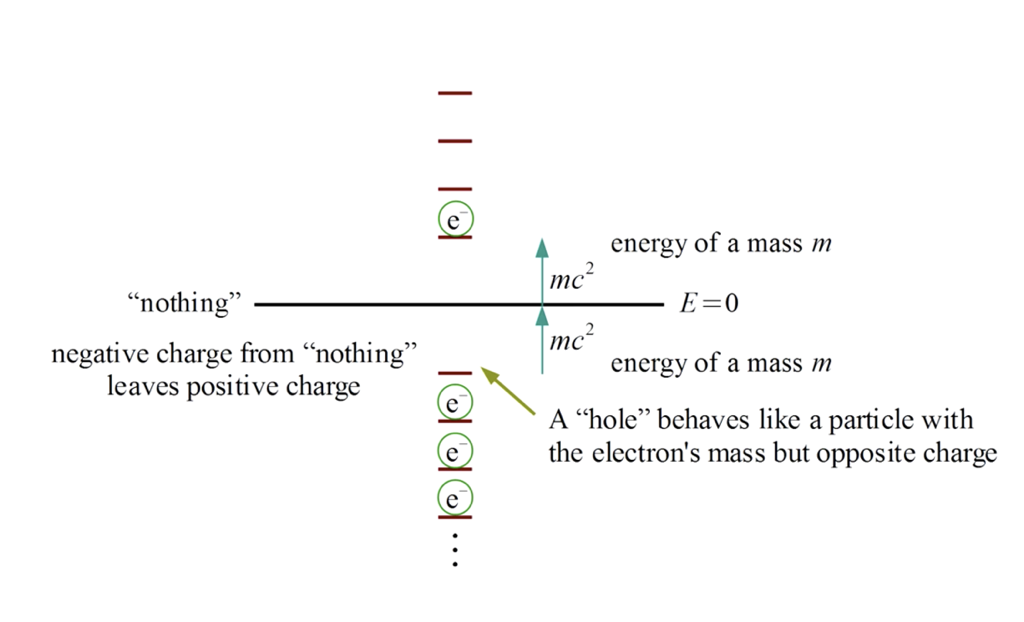
\includegraphics[scale=0.3]{negativeSea.png}
\end{frame}

%\begin{frame}
%\frametitle{Relativistic quantum mechanics is not enough}
%
%\includegraphics[scale=0.3]{problemsRQM.png}
%\end{frame}
%
%\begin{frame}
%\frametitle{QFT for pedestrians}
%
%\includegraphics[scale=0.3]{FeymanDiagram.png}
%\end{frame}
%
%\begin{frame}
%\frametitle{QED diagrams}
%
%\includegraphics[scale=0.3]{QEDDiagrams.png}
%\end{frame}







%
\begin{frame}
\frametitle{Dirac revisited}
In modern QED we interpret the solutions of the Dirac equation as a 4-dimensional spinor $\psi$:
\[
\psi = \mqty(\psi_1 \\ \psi_2 \\ \psi_2 \\ \psi_4) = \mqty(\phi \\ \chi)
\]
where $\phi =  \mqty(\phi_1 \\ \phi_2)$ represents a particle (with two spin states) and
$\chi =  \mqty(\chi_1 \\ \chi_2)$ represents an antiparticle (also with two spin states).

Notice also that the four $\gamma$~matrices, found before, are not unique. Any set that satisfy the anticommutation relations (Clifford algebra) can be used:

\begin{empheq}[box=\fbox]{align}
\{\gamma^\mu, \gamma^\nu\} = 2 g^{\mu\nu} \nonumber
\end{empheq}

\end{frame}

\begin{frame}
\frametitle{Dirac equation using Weyl representation of the $\gamma$~matrices}
\[
\gamma^0  = \mqty(0 & I \\ I & 0),\,\,\, \gamma^i  = \mqty(0 & -\sigma^i \\ \sigma^i  & 0)
\]
Then the Dirac equation becomes:
\[
\left[ E  \mqty(0 & I \\ I & 0) - \mqty(0 & -\va{p}\cdot\va{\sigma} \\ \va{p}\cdot\va{\sigma}  & 0) -m \right]
 \mqty(\phi \\ \chi) = 0
\]
which solves into two equations:
 \begin{empheq}[box=\fbox]{align}
(E +  \va{p}\cdot\va{\sigma}) \chi - m \phi & = 0 \nonumber \\
(E -  \va{p}\cdot\va{\sigma}) \phi - m \chi & = 0 \nonumber
\end{empheq}

The first equation represents particles (electrons) while the second represent antiparticles (positrons). In each equation, the helicity states (left-handed and right handed) are coupled through the particle mass. Notice that we can "assign" unambiguously one solution to {\it matter} ($e^-$) and another to {\it antimatter} ($e^+$), given the fact, dictated by nature, that positrons and electrons are electrically charged particles (with opposite charges). 

\end{frame}



%
%\begin{frame}
%\frametitle{Massless particles}
%In the limit of $m \rightarrow 0$~ these two equations decouple and we obtain
%two states with definite helicity:
% \begin{empheq}[box=\fbox]{align}
%(E +  \va{p}\cdot\va{\sigma}) \chi  & = 0 \nonumber \\
%(E -  \va{p}\cdot\va{\sigma}) \phi  & = 0 \nonumber
%\end{empheq}
%Notice that we have now only two degrees of freedom, since the particle has negative helicity and the antiparticle positive helicity. \alert{Massless particles have well defined helicity}. Thus, a massless $e^-$ is left-handed and a massless $e^+$ is right-handed. 
%
%\end{frame}


\begin{frame}
\frametitle{The need of Quantum Field Theory}
In spite of the heroic efforts of Dirac and others, RQM is not enough to describe elementary particles. The Dirc equation describes a single electron. Positrons need to be introduced by a sort of magical incantation (the negative sea state). In short, RQM cannot predict creation and annihilation of particles. 

Quantum Electrodynamics (QED) was eventually developed as the first Quantum Field Theory (QFT), capable of describing such creation and annihilation of particles. In QED, it is not only the photons that are quanta of a field but also the charged particles, like the electrons and positrons. The fields are operators that create and annihilate their quanta. \alert{Thus $\psi(x)$~is no longer interpreted as a waveform that describes probability but as an operator that creates a particle in point $x$~and destroys an antiparticle in $x$ ($\bar{\psi}(x)$~will create an antiparticle in point $x$~and destroy antiparticle in $x$)}.

The Lagrangian of the free Dirac field $\psi$~is given by:

\begin{empheq}[box=\fbox]{align}
  L = \bar{\psi}(i\gamma^\mu \partial_\mu -m)\psi  \nonumber
\end{empheq}

where $\bar{\psi} = \psi^\dagger \gamma^0$. Varying the Lagrangian yields back the Dirac equation. 
%The $\gamma$~matrices found by Dirac were complex. This means that the spinor field $\psi$~must also be complex. This makes sense from the point of view of field theory as a complex field would create particles and annihilate anti-particles while its complex conjugate would create anti-particles and annihilate particles. However, as we shall see, Majorana found an alternative. 

\end{frame}


\begin{frame}
\frametitle{Feynman Diagrams}
\begin{columns}
\column{0.4\textwidth}
\includegraphics[scale=0.3]{img/FeynmanD2.png}
 
\column{0.5\textwidth}
Feynman diagrams: ``pictures'' whose lines are world-lines of the particles in the space-time. They are representations of mathematical expressions of scattering or decay amplitudes. We cannot do the math here, but the diagrams suggest nicely the underlying physics. 

\end{columns}
\end{frame}
\begin{frame}
\includegraphics[scale=0.3]{img/FeynmanD3.png}

\end{frame}
%

%\input{lsc/diracRevisited.tex}

%\input{lsc/neutrinos.tex}

%\begin{frame}
\frametitle{A symmetric electron-positron theory (1937)}
\begin{columns}
\column{0.35\textwidth}
\includegraphics[scale=0.32]{img/MajoranaPaper.png}
\column{0.35\textwidth}
We show that it is possible to achieve complete formal symmetrization in the electron and positron quantum theory by means of a new quantization process. The meaning of Dirac equations is somewhat modified and {\bf it is no more necessary to speak of negative-energy states; nor to assume, for any other type of particles, especially neutral ones, the existence of antiparticles, corresponding to the ``holes'' of negative energy.}
\end{columns}
\end{frame}

%\begin{frame}
%\frametitle{An unpleasant symmetry}
%\begin{itemize}
%\item ``The interpretation of the so called ``negative energy states'' proposed by Dirac leads, as it is well known, to a substantially symmetric description of electron and positrons... but it looks to us important, in view of possible extensions, that the notion itself of negative energy state be abandoned." 
%\item ``Indeed, we shall see that to be perfectly possible to build, in the most natural way, a theory of the neutral elementary particles without negative states."
%\item ``The new approach allows not only to give a symmetric form to the electron-positron theory, but also to build a substantially novel theory for the particles deprived of electric charge."
%\item ``it is probably not yet possible to ask to the experience to decide between this new theory and the simple extension of the Dirac equations to the neutral particles."
%\end{itemize}
% 
% \alert{VOW!}
% 
%\begin{itemize}
%\item At the time the neutrino had not yet been discovered. 
%\item Even if in those times the only known ``charge'' was the electric charge, Majorana implicitly assumed particles deprived of \alert{all the possible charges}. 
%%\item Eighty years later we have not yet been able to decide between Dirac and Majorana theories.
%%\item But we hope we will be able to tell in maybe another ten or twenty years.
%\end{itemize}
%\end{frame}

\begin{frame}
\frametitle{Majorana's approach}
Majorana questioned whether it was necessary for spin-1/2 particles to have equations that involved complex numbers. What was required were gamma matrices that still satisfy the Clifford algebra but were purely imaginary. Majorana found such constructions in terms of the Pauli matrices:
\[
\gamma^0 = \mqty(0 & \sigma_2 \\ \sigma_2 & 0), \,\,\,
\gamma^1 = \mqty(i \sigma_1 & 0 \\ 0 & i \sigma_1), \,\,\,
\gamma^2 = \mqty(0 & -\sigma_2 \\ \sigma_2 & 0), \,\,\,
\gamma^4 = \mqty(i \sigma_3 & 0 \\ 0 & i \sigma_3)
\]
Recall that $\sigma_1, \sigma_3$~are real, while $\sigma_2$~is complex. Thus, all the Majorana gamma matrices are complex. But then, the Majorana spinor $\psi_M$~must be real \alert{and is therefore invariant to charge conjugation}. The derived field theory can be constructed from one type of operator. Therefore, the particles created \alert{are fermions that are their own antiparticles}.
\end{frame}
%
%\begin{frame}
%\frametitle{Dirac revisited}
%In modern QED we interpret the solutions of the Dirac equation as a 4-dimensional spinor $\psi$~is a:
%\[
%\psi = \mqty(\psi_1 \\ \psi_2 \\ \psi_2 \\ \psi_4) = \mqty(\phi \\ \chi)
%\]
%where $\phi =  \mqty(\phi_1 \\ \phi_2)$ represents a particle (with two spin states) and
%$\chi =  \mqty(\chi_1 \\ \chi_2)$ represents an antiparticle (also with two spin states).
%\end{frame}
%
%\begin{frame}
%\frametitle{Dirac equation using Weyl representation of the $\gamma$~matrices}
%\[
%\gamma^0  = \mqty(0 & I \\ I & 0),\,\,\, \gamma^i  = \mqty(0 & -\sigma^i \\ \sigma^i  & 0)
%\]
%Then the Dirac equation becomes:
%\[
%\left[ E  \mqty(0 & I \\ I & 0) - \mqty(0 & -\va{p}\cdot\va{\sigma} \\ \va{p}\cdot\va{\sigma}  & 0) -m \right]
% \mqty(\phi \\ \chi) = 0
%\]
%which solves into two equations:
% \begin{empheq}[box=\fbox]{align}
%(E +  \va{p}\cdot\va{\sigma}) \chi - m \phi & = 0 \nonumber \\
%(E -  \va{p}\cdot\va{\sigma}) \phi - m \chi & = 0 \nonumber
%\end{empheq}
%
%The first equation represents particles (electrons) while the second represent antiparticles (positrons). In each equation, the helicity states (left-handed and right handed) are coupled through the particle mass. Notice that we can "assign" unambiguously two solutions two {\it matter} ($e^-$) and two solutions to {\it antimatter} ($e^+$), given the fact, dictated by nature that positrons and electrons are electrically charged particles (with opposite charges). 
%\end{frame}
%
%\begin{frame}
%\frametitle{Electron mass in modern QFT: coupling helicity states to the Higgs Field}
%\includegraphics[scale=0.30]{img/ElectronMass.png}
%\end{frame}
%
%
%\begin{frame}
%\frametitle{Massless particles}
%In the limit of $m \rightarrow 0$~ these two equations decouple and we obtain
%two states with definite helicity:
% \begin{empheq}[box=\fbox]{align}
%(E +  \va{p}\cdot\va{\sigma}) \chi  & = 0 \nonumber \\
%(E -  \va{p}\cdot\va{\sigma}) \phi  & = 0 \nonumber
%\end{empheq}
%Notice that we have now only two degrees of freedom, since the particle has negative helicity and the antiparticle positive helicity. 
%
%\end{frame}
%
%
\begin{frame}
\frametitle{Majorana insight}
Majorana proposed an alternative to the two-coupled, two-component Dirac equation, namely two independent, relativistic, two-component equations:

 \begin{empheq}[box=\fbox]{align}
(E +  \va{p}\cdot\va{\sigma}) \chi - m \epsilon \chi^* & = 0 \nonumber \\
(E -  \va{p}\cdot\va{\sigma}) \phi - m \epsilon \phi^* & = 0 \nonumber
\end{empheq}
where
\[
\epsilon = i \sigma_2 = \mqty(0 & I \\ -I & 0)
\]
If we compare with the Dirac equation:
 \begin{empheq}[box=\fbox]{align}
(E +  \va{p}\cdot\va{\sigma}) \chi - m \phi & = 0 \nonumber \\
(E -  \va{p}\cdot\va{\sigma}) \phi - m \chi & = 0 \nonumber
\end{empheq}
It's obvious that both equations are identical for $m=0$. In the Standard Model neutrinos are assumed to be massless and thus both theories are identical. Instead, if neutrinos are massive they are not. The remarkable thing about Majorana equation is that it is constructed only with the $\phi$ (or the $\chi$ for the second equation), thus eliminating two degrees of freedom. 
\end{frame}

%\begin{frame}
%\frametitle{Is the neutrino its own antiparticle?}
%\alert{A particle is its own antiparticle if we can reverse all its charges without effect}. Obviously electrons cannot be their own antiparticles, but Dirac neutrinos are also not their own antiparticles, as explicit in the construction of the bi-spinor that separates particles ($\phi$) and antiparticles ($\chi$).
%
%Given a spinor $\phi$~representing a particle, the charge-conjugate spinor representing an antiparticle is:
%
% \begin{empheq}[box=\fbox]{align}
% \phi^C & = C \gamma^0 \phi^*\nonumber
%\end{empheq}
%%\[
%%\phi^C = C \gamma^0 \phi^* 
%%\]
%where $\phi^*$~is the complex conjugate of $\phi$ and the charge conjugation matrix $C$~can be written in the Weyl representation as:
%\[
%C = \mqty(-i\sigma_2 & 0 \\ 0 & i\sigma_2), \,\,\, C \gamma^0 = \mqty(0 & -i\sigma_2 \\ i \sigma_2 & 0)
%\] 
%\end{frame}
%
%\begin{frame}
%For a Majorana spinor $\phi  \mqty(\phi \\ i \sigma_2 \phi^*)$:
%\begin{empheq}[box=\fbox]{align}
%\phi^C & = C \gamma^0 \phi^* =  \mqty(0 & -i\sigma_2 \\ i \sigma_2 & 0) \mqty(\phi^* \\ -i \sigma_2 \phi) \\
%& =\mqty(-i^2 \sigma^2 \phi \\ i \sigma_2 \phi^*) = \mqty(\phi \\ i \sigma_2 \phi^*) = \phi
%\nonumber
%\end{empheq}
%Thus, \alert{a Majorana particle is identical to its antiparticle.}
%\end{frame}
%
%\begin{frame}
%\frametitle{Majorana neutrinos violate lepton number}
%\includegraphics[scale=0.08]{muonDecay.png}
%
%Lepton number counts the total number of leptons and anti-leptons involved in a weak interaction which must be zero. For example, in the
%decay of $\mu$~above, the disappearance of the $\mu^-$~ (a lepton) is compensated with the appearance of a $\nu_\mu$~(also a lepton), while the appearance of $e^-$~(a lepton) is compensated with the
%appearance of a $\bar{\nu_e}$~(an anti-lepton). On the contrary, Majorana neutrinos have no lepton number. As such they may induce processes violating lepton number conservation.
%
%In most processes involving neutrinos the energy of the process is very large compared with the (tiny) neutrino mass. In practice we approach the limit $m=0$~and Dirac and Majorana become impossible to distinguish. 
%
%\end{frame}
%

\begin{frame}
\frametitle{Majorana neutrinos}
\includegraphics[scale=0.30]{img/MajoranaNeutrinosCartoon.png}
\end{frame}

%\begin{frame}
%\frametitle{Majorana mass}
%\includegraphics[scale=0.30]{img/MajoranaMass.png}
%\end{frame}

\begin{frame}
\frametitle{Majorana and Dirac neutrinos}
\includegraphics[scale=0.4]{img/DiracVsMajorana2.pdf}
\end{frame}

\begin{frame}
\frametitle{Dirac or Majorana?}
\begin{columns}
\column{0.45\textwidth}
\includegraphics[scale=0.10]{img/dirac_4.jpg}

\begin{empheq}[box=\fbox]{align}
(E +  \va{p}\cdot\va{\sigma}) \chi - m \phi & = &  0 \nonumber \\
(E +  \va{p}\cdot\va{\sigma}) \chi - m \epsilon \chi^* & = & 0 \nonumber
\end{empheq}

\column{0.5\textwidth}
\includegraphics[scale=0.30]{img/Majorana.jpg}

\begin{empheq}[box=\fbox]{align}
(E +  \va{p}\cdot\va{\sigma}) \chi - m \epsilon \chi^* & = 0 \nonumber \\
(E -  \va{p}\cdot\va{\sigma}) \phi - m \epsilon \phi^* & = 0 \nonumber
\end{empheq}

\end{columns}
\end{frame}

\begin{frame}
\frametitle{Deus ex machina}
\includegraphics[scale=0.30]{img/DeusExMachina.png}
\end{frame}

\begin{frame}
\frametitle{Dirac neutrino mass: Deus ex machina}
\includegraphics[scale=0.30]{img/SmallNeutrinoMasses.png}
\end{frame}

%\begin{frame}
%\frametitle{Majorana neutrinos}
%\includegraphics[scale=0.30]{img/MajoranaNeutrinosCartoon.png}
%\end{frame}
%

\begin{frame}
\frametitle{Electron mass in modern QFT: coupling helicity states to the Higgs Field}
\includegraphics[scale=0.30]{img/ElectronMass.png}
\end{frame}

\begin{frame}
\frametitle{Massive neutrinos can be described by Dirac's equation}
\begin{columns}
\column{0.30\textwidth}
%\includegraphics[scale=0.35]{img/NeutrinoHelicity.png}


 \begin{empheq}[box=\fbox]{align}
(E +  \va{p}\cdot\va{\sigma}) \chi - m \phi & = 0 \nonumber \\
(E -  \va{p}\cdot\va{\sigma}) \phi - m \chi & = 0 \nonumber
\end{empheq}


However, unlike the case of the electron, we don't have a "label" (e.g., the electric charge) to separate the unambiguously the particle and the antiparticle. 

\column{0.65\textwidth}
\includegraphics[scale=0.24]{img/NeutrinoMassDirac.png}

\end{columns}
\end{frame}

\begin{frame}
\frametitle{Majorana mass may solve the problem of scale}
\includegraphics[scale=0.30]{img/MajoranaMass.png}
\end{frame}

%\begin{frame}
%\includegraphics[scale=0.30]{img/Effective.png}
%\end{frame}



\begin{frame}
\frametitle{The mystery of the missing antimatter}
\includegraphics[scale=0.30]{img/MissingAntiMatter.png}
\end{frame}

\begin{frame}
\frametitle{CP violation and Majorana neutrinos}
\includegraphics[scale=0.30]{img/CP.png}
\end{frame}

\begin{frame}
\frametitle{We are the leftovers}
\includegraphics[scale=0.30]{img/MissingUniverse.png}
\end{frame}
%

\begin{frame}
\frametitle{A formula for the Universe}
\includegraphics[scale=0.30]{img/formulaUniverse.png}
\end{frame}




%\input{energyAndSpinProjections.tex}
%\input{highEnergySolutions.tex}


%\input{lsc/diracRevisited.tex}
%%\begin{frame}
%\frametitle{Massless particles and helicity}
%\begin{columns}
%\column{0.5\textwidth}
%\includegraphics[scale=0.35]{img/NeutrinoHelicity.png}
%
%Helicity is the spin projection in the direction of motion.
%\[
%h = \frac{\va{\sigma}\cdot \va{p}}{p}
%\]
%In the limit of $m \rightarrow 0$~ Dirac's equation(s) decouple in 
%two states with definite helicity:
% \begin{empheq}[box=\fbox]{align}
%(E +  \va{p}\cdot\va{\sigma}) \chi  & = 0 \nonumber \\
%(E -  \va{p}\cdot\va{\sigma}) \phi  & = 0 \nonumber
%\end{empheq}
%The particle has negative helicity and the antiparticle positive helicity. \alert{Massless particles have well defined helicity}. \column{0.5\textwidth}
%
%\includegraphics[scale=0.30]{img/neutrinoBoost2.png}
%
%For massive particles, helicity depends on the reference frame. One can always jump into a reference system faster than that of the particle and see its helicity flip.
%
%But massless particles travel at the speed of light and cannot be overtaken. The helicity becomes a constant of motion. 
%\end{columns}
%
%\end{frame}
%
%\begin{frame}
%\frametitle{Neutrino oscillations}
%%\begin{columns}
%%\column{0.4\textwidth}
%\includegraphics[scale=0.30]{img/neutrinoOscillations.png}
%%\column{0.4\textwidth}
%%\begin{block}{}
%
%Neutrino oscillation experiments (a story to be told some other time) have established that neutrinos are massive. Their mass is, however, very small. This is the reason why parity experiments found the neutrino to be left handed, since the effects associated to their masses are of the order of $m/E$~where $m$~is the mass of the neutrino (tiny) and $E$~the energy of the process (much larger). 
%
%\alert{But how do we give a mass to the neutrinos?} 
%
%%\end{block}
%%\end{columns}
%\end{frame}
%
%\begin{frame}
%\frametitle{Electron mass}
%\includegraphics[scale=0.30]{img/ElectronMass.png}
%\end{frame}

\begin{frame}
\frametitle{Neutrino mass (Dirac recipe)}
\includegraphics[scale=0.30]{img/NeutrinoMassDirac.png}
\end{frame}

\begin{frame}
\frametitle{Deus ex machina}
\includegraphics[scale=0.30]{img/DeusExMachina.png}
\end{frame}

\begin{frame}
\frametitle{Dirac neutrino mass: Deus ex machina}
\includegraphics[scale=0.30]{img/SmallNeutrinoMasses.png}
\end{frame}

\begin{frame}
\frametitle{Majorana neutrinos}
\includegraphics[scale=0.30]{img/MajoranaNeutrinosCartoon.png}
\end{frame}

\begin{frame}
\frametitle{Majorana mass}
\includegraphics[scale=0.30]{img/MajoranaMass.png}
\end{frame}

\begin{frame}
\includegraphics[scale=0.30]{img/Effective.png}
\end{frame}

\begin{frame}
\frametitle{The mystery of the missing antimatter}
\includegraphics[scale=0.30]{img/MissingAntiMatter.png}
\end{frame}

\begin{frame}
\frametitle{CP violation and Majorana neutrinos}
\includegraphics[scale=0.30]{img/CP.png}
\end{frame}

\begin{frame}
\frametitle{We are the leftovers}
\includegraphics[scale=0.30]{img/MissingUniverse.png}
\end{frame}
%

\begin{frame}
\frametitle{A formula for the Universe}
\includegraphics[scale=0.30]{img/formulaUniverse.png}
\end{frame}











\end{document}